\pagestyle{fancy}
\chapter{El problema inverso}
\lhead{\thepage}
\rhead{\textit{El problema inverso}} 
\vspace{0.01\textheight}
\label{sec:inverso}
\pagebreak

En las secciones previas abordamos el problema {\bf directo} de transporte 
de radiación en la materia mediante la ETR. 
En este problema los parámetros ópticos $a(\x)$, $b(\x)$, la función  
de fase $\eta(\hth\cdot \hth')$, la velocidad de la luz en el medio participante 
$c$, las fuentes internas $s(\x,\hth,t)$ y las condiciones iniciales y de contorno 
son datos. Se busca encontrar la solución $\ut$ a la Ecuación~\eqref{eq:RTE}.

En el problema {\bf inverso}, alguno de los parámetros son conocidos, 
 y se dispone de mediciones experimentales  
obtenidas por detectores. 
A partir de estas mediciones, 
el objetivo de este problema es la reconstrucción de las características del medio, incluyendo 
al resto de los parámetros desconocidos. 

En el contexto de esta Tesis, reconstruiremos, para distintos problemas, 
 el coeficiente de absorción $a(\x)$ en tomografía óptica. Esto encuentra numerosas aplicaciones. Por ejemplo, 
 para aplicaciones médicas, identificación de tumores~\cite{Zhu2005,Zhu2010,Fujii2016b}, imágenes funcionales del cerebro~\cite{Boas2001,bluestone2001,Arridge1999}, 
y la caracterización de diferentes constituyentes del tejido.
En el caso de tomografía por fluorescencia y tomografía de bioluminiscencia~\cite{Klose2005,Klose2009,Ren2010},
 se intentan determinar 
las fuentes $s(\x,\hth,t)$ en la Ec.~\eqref{eq:RTE}. 
Estas fuentes están relacionadas a los coeficientes de absorción de los 
cromóforos y fluoróforos. 
En aplicaciones de diagnóstico y monitoreo para el tratamiento de tumores, 
se asume cierta información previa  
del coeficiente de dispersión 
$b(\x)$. Esta se obtiene, generalmente, mediante técnicas de 
 imágenes de alta resolución~\cite{Althobaiti2017,Guven2003}, \eg Resonancia Magnética, que poseen ciertas limitaciones.   
 El alto costo y la baja disponibilidad 
de este tipo de aparatos dificulta el seguimiento de tratamientos  
asistidos por diagnóstico de imágenes. 
Por el contrario, los dispositivos 
utilizados en tomografía óptica son portables, facilitando su disponibilidad. 
Las imágenes permiten determinar regiones, 
como por ejemplo ciertos tejidos óseos, o 
el aire en la traquea del cuello humano, en las cuales 
los coeficientes de absorción toman valores conocidos.  
Adicionalmente, estas sirven para imponer cotas superiores e inferiores 
de $a(\x)$, lo que permite restringir el espacio de funciones donde se busca minimizar 
la función objetivo. Si bien en 
este trabajo nos enfocamos en la reconstrucción del coeficiente 
de absorción, los algoritmos y las estrategias propuestas 
pueden ser fácilmente generalizadas para otros parámetros. 

En la figura~\ref{fig:esquemainv} 
esquematizamos los problemas directos e inverso, tal como son 
tratados en esta Tesis. 

\begin{figure}[h!]
\centering
  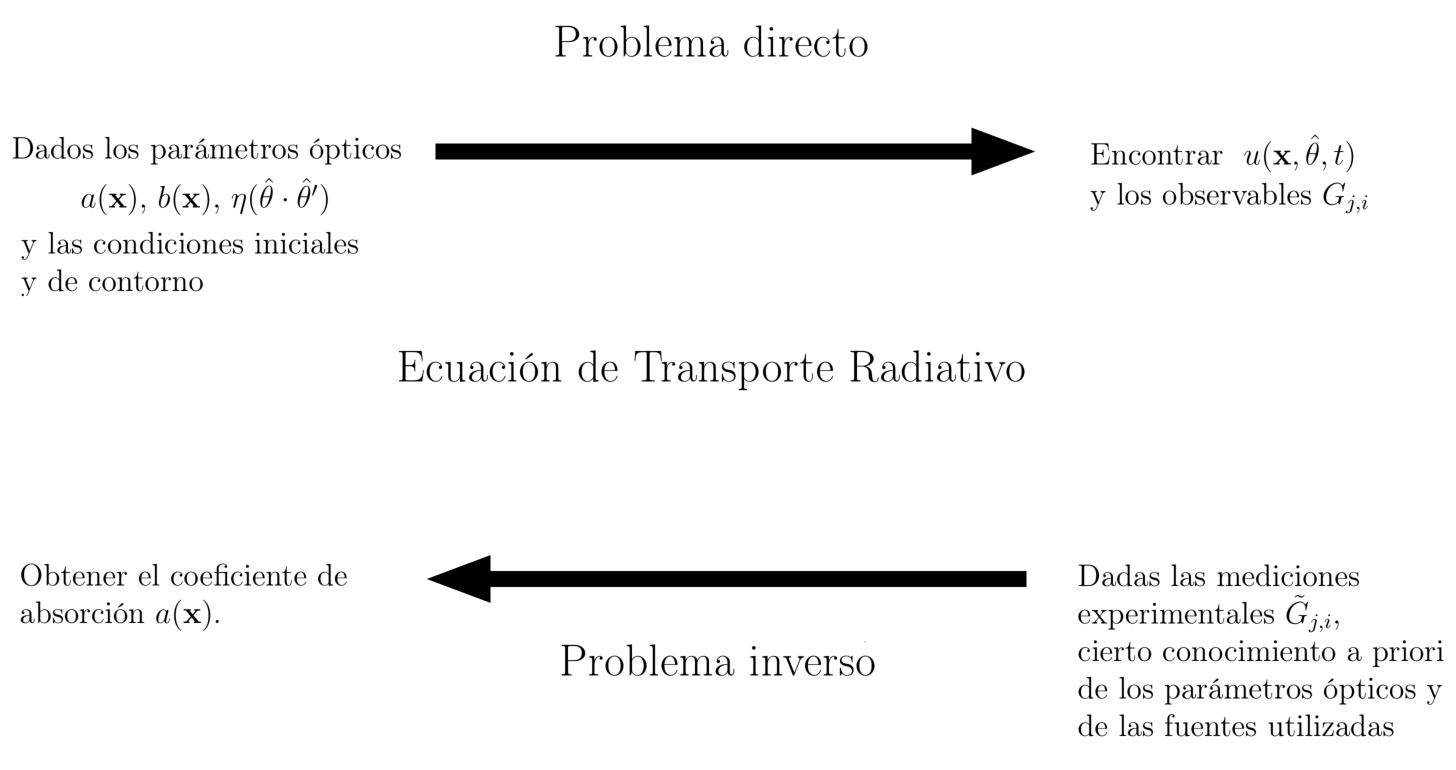
\includegraphics[width=\linewidth]{figuras/inv.pdf}\\
  \caption{
Grafico esquemático de los problemas directo e inverso.}
 \label{fig:esquemainv}
\end{figure}
Para la resolución del problema inverso, utilizamos el esquema \textit{MOBIR}, 
presentado en la sección siguiente. 

\pagebreak

\section{El esquma \textit{MOBIR}}

\begin{wrapfigure}{l}{0.48\textwidth}
  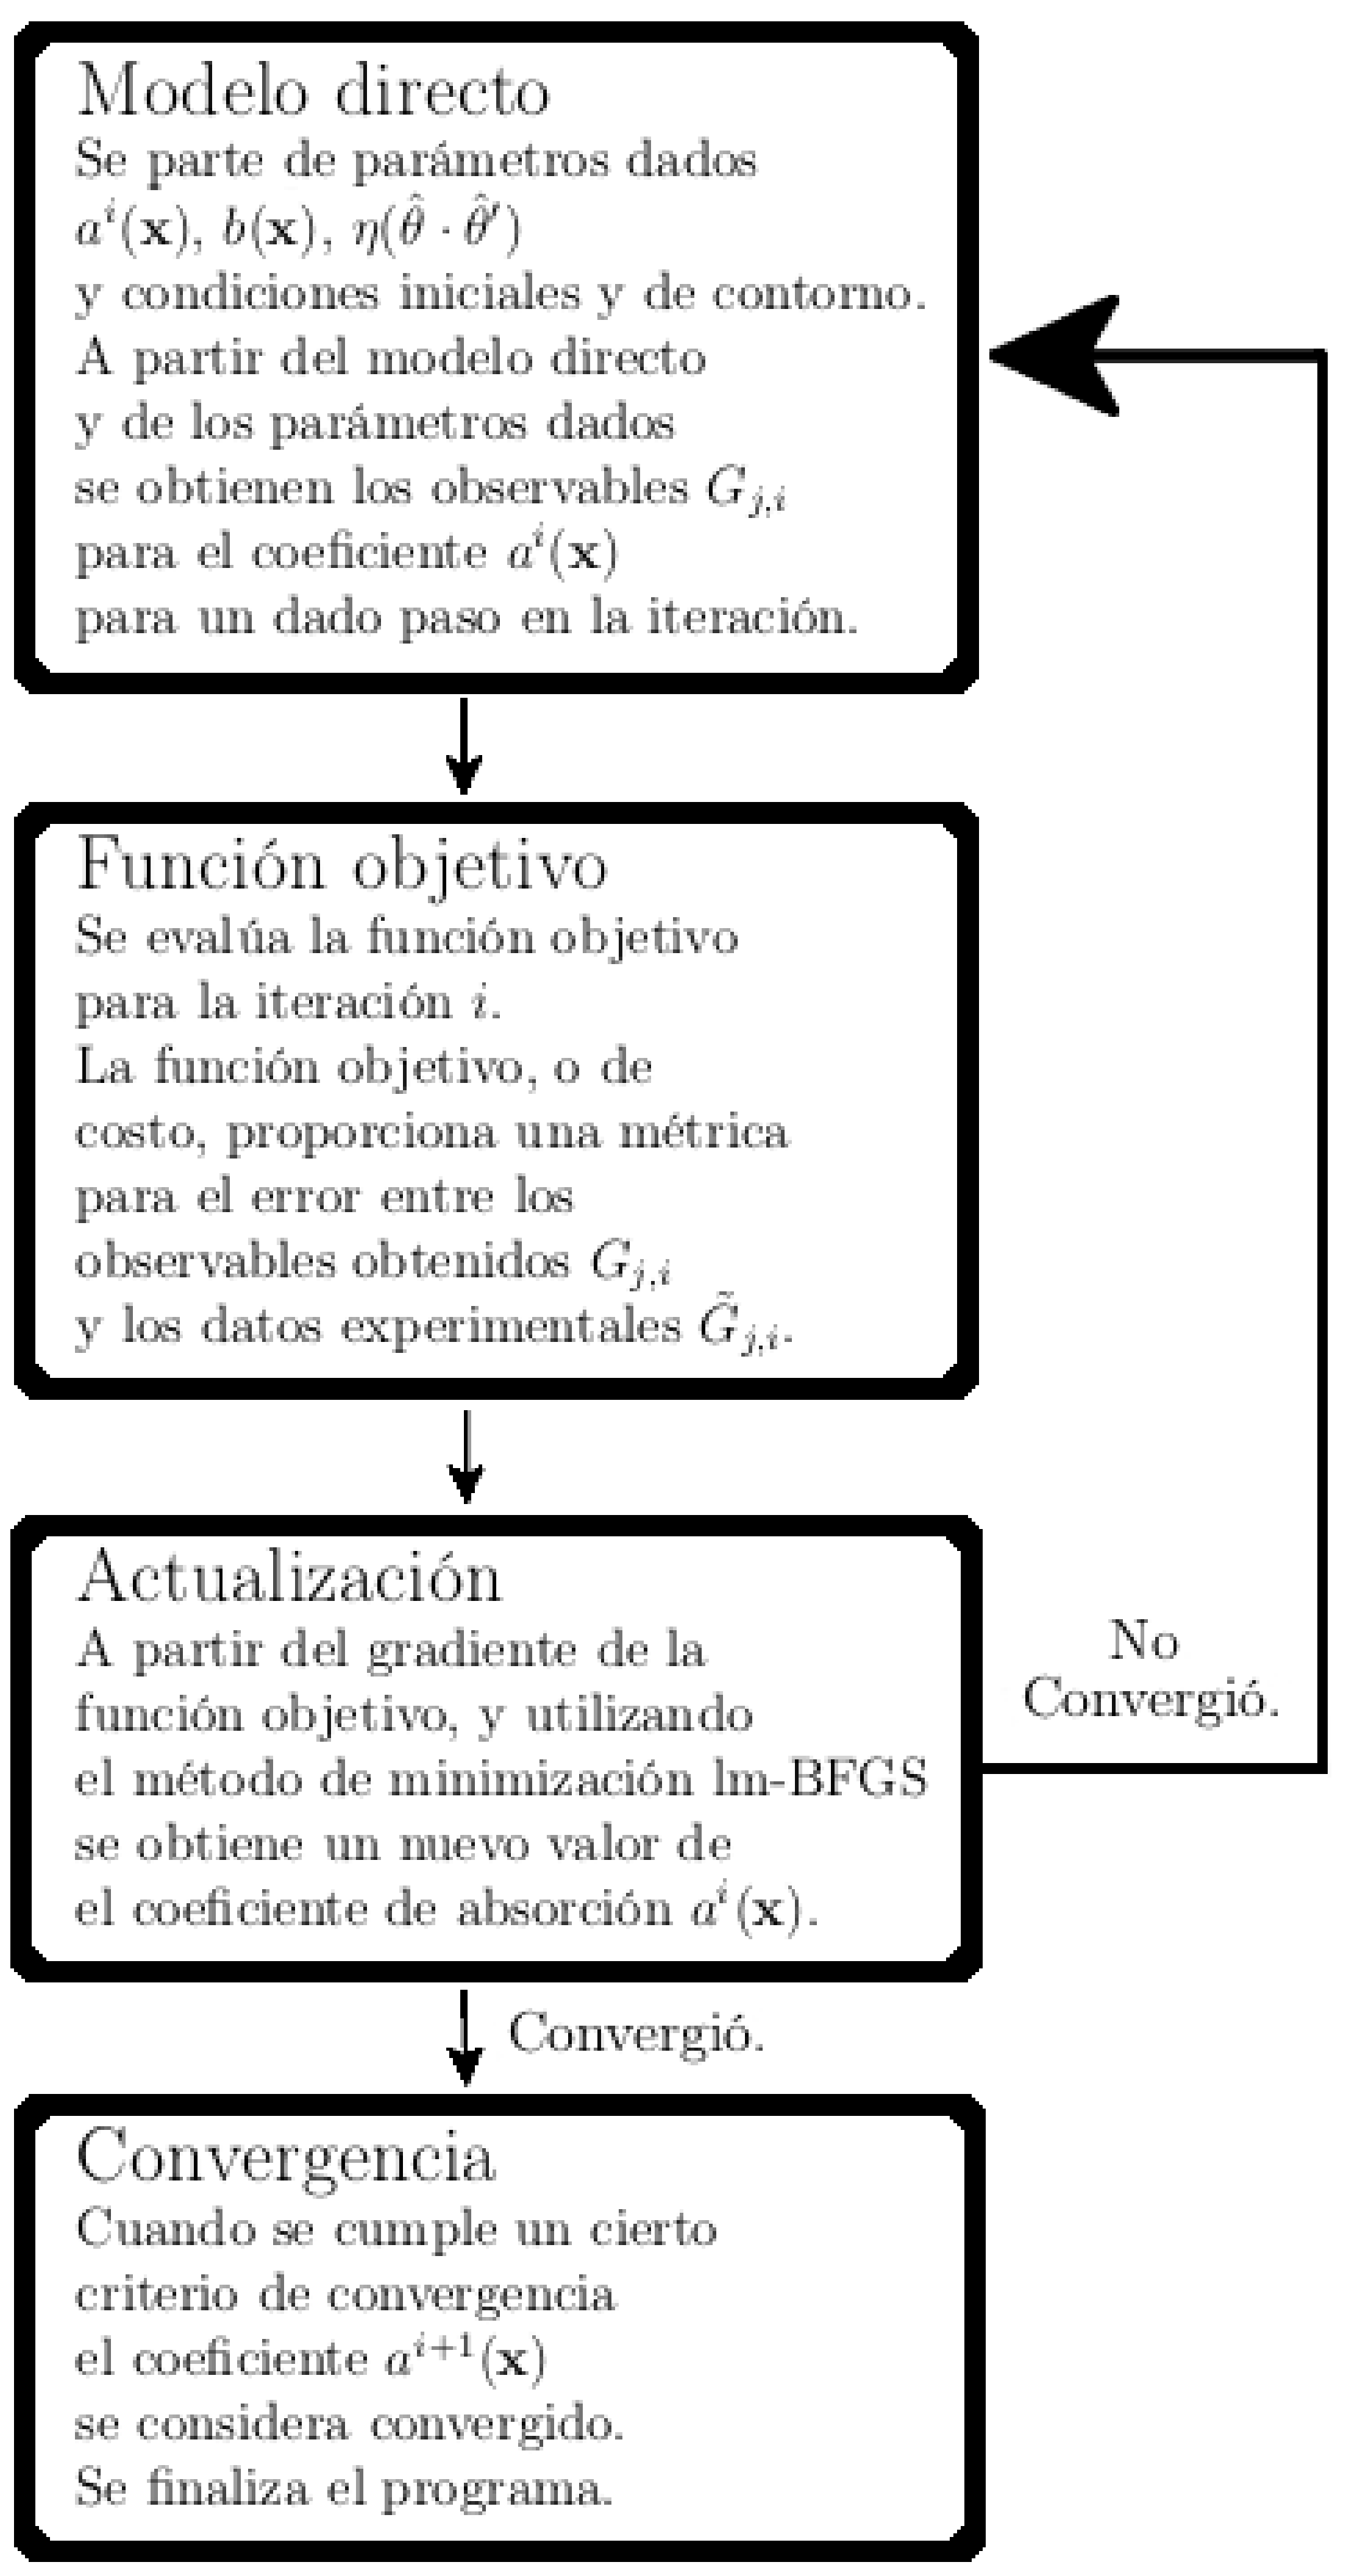
\includegraphics[width=0.48\textwidth]{figuras/mobir.eps}\\
  \caption{Esquema  MOBIR.}
 \label{fig:mobir}
\end{wrapfigure}

En este trabajo desarrollamos un algoritmo tipo MOBIR~\cite{Hielscher1999,Kim2010} (del inglés, {\em Model Based Iterative Image  
Reconstruction}). Este esquema se basa en un modelo físico, y un método de minimización 
iterativo para la reconstrucción del parámetro deseado en el problema inverso. 
Como se muestra en la Figura~\ref{fig:mobir}, en este esquema, el modelo directo es utilizado para obtener los observables simulados. Luego se evalúa el error entre los datos experimentales y los simulados por medio de la función objetivo. A continuación, utilizando un método de minimización, se actualiza el coeficiente $a^{i+1}(\x)$ a 
  ser utilizado en la iteración subsiguiente. Este 
  procedimiento se repite hasta converger.
El modelo físico utilizado es la Ecuación de Transporte Radiativo~\eqref{eq:RTE}. 
Para la minimización del funcional objetivo (que será introducido en una sección posterior) 
emplearemos el método de minimización 
de Broyden--Fletcher--Goldfarb--Shanno (BFGS) con uso de memoria reducido 
(lm--BFGS, de su sigla en inglés)~\cite{Byrd1995}. Este puede ser considerado un caso particular 
de los métodos cuasi--Newton~\cite{Nocedal2006,Klose2003QN,Ren2006}.
El problema inverso en tomografía óptica es resuelto como un problema de optimización 
no lineal. A partir de un coeficiente de absorción $a^0(\x)$ inicial, 
se actualiza su valor  en cada paso de la iteración $i$, 
mediante el método lm--BFGS según~\cite{Klose2003QN}
\begin{equation}
\mathbf{a}^{i+1}(\x)=\mathbf{a}^{i}(\x)+\alpha^i  \mathbf{d}^i(\x)
\label{eq:update}
\end{equation}
donde $\mathbf{a}^{i}(\x)$ es el 
vector obtenido a partir del coeficiente de absorción $a(\x)$, 
con la variable $\x$ discretizada, $\alpha^i$ es el largo del paso de Newton (consideraremos, por simplicidad $\alpha^i=1$, 
en general $\alpha^i$ debe satisfacer las condiciones de Wolfe~\cite{Nocedal2006}). En el caso del método de Newton (o {\em steepest descent}), la dirección de 
descenso vendrá dada por el gradiente $\mathbf{d}^i=-\nabla_a g[\mathbf{a}^{i}]$, donde la función objetivo $g$ será definida posteriormente. 
En el contexto de esta Tesis la dirección de descenso será determinada por el método lm--BFGS, 
muy eficiente en tomografía óptica~\cite{Klose2003QN,Ren2006,Prieto2017}. 

\section{El método de minimización BFGS}
\label{sec:BFGS}
Siguiendo a Nocedal~\cite[Cap. 2 y 6]{Nocedal2006}, el método BFGS parte de considerar la expansión de 
Taylor a segundo orden de la función objetivo $g[\mathbf{a}]$
que buscamos minimizar
\begin{equation}
g[\mathbf{a}^i+ \mathbf{d}^i]\approx g[\mathbf{a}^i]+ (\mathbf{d}^i)^T \nabla_a g[\mathbf{a}^i]+
\frac{1}{2}(\mathbf{d}^i)^T \nabla_a^2 g[\mathbf{a}^i+t\mathbf{d}^i] \mathbf{d}^i\equiv m(\mathbf{d}^i).
\label{eq:Taylor}
\end{equation}
donde $t \in (0,1)$, y $(\mathbf{d}^i)^T$ indica el vector traspuesto a $\mathbf{d}^i$.

Exigiendo que se anule la derivada de $m(\mathbf{d^i})$, se llega la dirección de Newton, dada por
\begin{equation}
\mathbf{d}^i=-(\nabla_a^2 g^i )^{-1} \nabla_a g^i.
\label{eq:direccion}
\end{equation}
El principal obstáculo para la aplicación de la dirección de Newton radica en el cálculo de la inversa del Hessiano $\nabla_a^2 g^i$ de la función objetivo,  
que en tomografía óptica puede 
resultar extremadamente costoso, debido a la alta dimensionalidad de la ETR. 
Por este motivo, el método BFGS implementa una aproximación del Hessiano (mas concretamente, 
de la inversa del Hessiano) que 
es actualizada a cada paso de la iteración. 

Exigiendo que el gradiente de la Ecuación~\eqref{eq:Taylor} coincida con el gradiente de la función objetivo 
en los últimos dos iterandos sucesivos se llega a
\begin{equation}
\begin{split}
\begin{aligned}
\nabla_a^2 g[\mathbf{a}^{i+1}-\mathbf{a}^i]& \approx \nabla_a g[\mathbf{a}^{i+1}]  - \nabla_a g[\mathbf{a}^{i}].
\end{aligned}
\end{split}
\label{eq:Taylor4}
\end{equation}
Esta última relación nos permite aproximar el Hessiano utilizando las derivadas de 
la función objetivo obtenidas para dos iteraciones sucesivas. 
La inversa del Hessiano es aproximada exigiendo que se cumpla la relación~\eqref{eq:Taylor4}, que puede escribirse 
\begin{equation}
(B^{i+1})^{-1}y^i=s^i,
\label{eq:Taylor5}
\end{equation}
con $s_i=  \mathbf{a}^{i+1}-\mathbf{a}^{i}$ y $y^i=\nabla_a g[\mathbf{a}^{i+1}]  - \nabla_a g[\mathbf{a}^{i}]$. 
La fórmula BFGS para actualizar el Hessiano en cada iteración viene dada por~\cite{Nocedal2006}
\begin{equation}
(B^{i+1})^{-1}=(V^i)^T (B^{i})^{-1}V^i + \rho^i s^i (s^i)^T  ,
%B^{i}-\frac{B^{i}s^i (s^i)^T B^i }{(s^i)^TB^i s^i}+ \frac{y^i (y^i)^T}{(y^i)^T s^i}
\label{eq:HBFGS}
\end{equation}
la cual cumple la relación~\eqref{eq:Taylor5}, donde $\rho^i=\frac{1}{(y^i)^T s^i}$ 
y $V^i=\id - \rho^i y^i (s^i)^T$. 
La dirección de descenso, finalmente, se obtiene de la Ecuación~\eqref{eq:direccion} reemplazando 
el Hessiano por su aproximación $B^i$
\begin{equation}
\mathbf{d}^{i}=-(B^{i})^{-1} \nabla_a g[\mathbf{a}^i]. 
\label{eq:HBFGS2}
\end{equation}

\subsection{El método de uso de memoria limitada lm--BFGS}
\label{sec:lmBFGS}
En nuestro algoritmo para la resolución del problema inverso, el coeficiente 
de absorción es actualizado en cada iteración utilizando la relación 
\begin{equation}
\mathbf{a}^{i+1}(\x)=\mathbf{a}^{i}(\x)-(B^{i})^{-1} \nabla_a g[\mathbf{a}^i].
\label{eq:update2}
\end{equation}
La discretización de la inversa del Hessiano $(B^i)^{-1}$ se representa con una matriz,  
que para el problema 2D tiene $N_x \times N_y$ puntos. 
La manipulación y almacenamiento de esta matriz puede ser sumamente costosa. Por ello, 
 se utiliza una versión aproximada, en la cual sólo se almacenan los vectores $\{s^k, y^k\}$, 
$k=i-m,...,i-1$ para un dado número de puntos $m$ previos a la iteración $i$--esima. 
Se utiliza una aproximación inicial al Hessiano $(B^i)^{-1}_0$~\cite[Cap. 7]{Nocedal2006}
\begin{equation}
(B^i)^{-1}_0=\gamma^i \id,\quad \quad \gamma^i=\frac{(s^{i-1})^T y^{i-1}}{(y^{i-1})^Ty^{i-1}},
\label{eq:initHess}
\end{equation}
y de la Ecuación~\eqref{eq:HBFGS} se tiene la relación de recurrencia
\begin{equation}
\begin{split}
\begin{aligned}
(B^{i+1})^{-1}=&(V^{i-1})^T...V^{i-m})^T) (B^i)^{-1}_0 (V^{i-m}...V^{i-1})  \\
&+\rho^{i-m} (V^{i-1})^T...V^{i-m+1})^T)s^{i-m} (s^{i-m})^T(V^{i-m+1}...V^{i-1+1}) \\
&+\rho^{i-m+1} (V^{i-1})^T...V^{i-m+2})^T)s^{i-m+1} (s^{i-m+1})^T(V^{i-m+2}...V^{i-1}) \\
&+...\\
&+\rho^{i-1} s^{i-1} (s^{i-1})^T. 
\end{aligned}
\end{split}
\label{eq:HBFGSrec}
\end{equation}
de donde surge el algoritmo~\eqref{algbfgs}~\cite{Byrd1995,Nocedal2006}

\begin{algorithm}
\caption{lm-BFGS}\label{algbfgs}
\begin{algorithmic}[1]
\State dados $m$, $\mathbf{a}^i$, y $\nabla_a g[\mathbf{a}^i]$
\State  $q = \nabla_a g[\mathbf{a}^i]$
\State \textbf{para} $k=i-1,i-2,\ldots,i-m$ hacer 
\State \hskip 0.75em $\alpha^k  = \rho^k (s^k)^T q$,
\State \hskip 0.75em $q  = q- \alpha^k y^k$,
\State \textbf{terminar}
\State $r = (B_0^k)^{-1} q$,
\State \textbf{para} $k=i-m,i-m+1,\ldots,i-1$ hacer 
\State \hskip 0.75em $\beta  = \rho^k (y^k)^T r$,
\State \hskip 0.75em $r  = r+s^k(\alpha^k-\beta)$,
\State \textbf{terminar}
\State Finalizar programa, con $(B^k)^{-1}\nabla_a g[\mathbf{a}^k]=r$.
\end{algorithmic}
\end{algorithm}  
  
En esta Tesis utilizaremos el valor 
de $m=5$, partiendo de un coeficiente inicial $a^0(\x)$ dado 
por cierto conocimiento previo. En la Sec.~\ref{sec:inverseres}, esto se ejemplifica utilizando la imagen 
de resonancia magnética de un cuello humano.
Las cotas inferiores $a^l(\x)$ y superiores $a^u(\x)$ del coeficiente de absorción 
limitan el subespacio de soluciones posibles a $a^l(\x)\leq a^i(\x) \leq a^u(\x)$. 
Una condición física que debe cumplirse siempre es que la cota inferior 
no sea negativa. Las regiones a estudiar que se diferencian del medio 
conocido se denominan inclusiones. En aquellos tejidos donde se sabe 
que no habrán inclusiones, el coeficiente de absorción 
puede fijarse utilizando $a^l(\x) = a^u(\x)=a^0(\x)$, cuyo valor se obtiene de la información preliminar. Si, por la naturaleza del diagnóstico que se está realizando, 
se espera que una dada inclusión no 
se encuentre dentro de cierto tipo de tejido 
puede restringirse la minimización para excluirlo 
del cálculo. 
Esto ocurre, por ejemplo, en la traquea del cuello humano, que 
al estar llena de aire, no puede contener 
un tumor en su interior.
Adicionalmente, se conocen cotas para el tipo de inclusión 
que se estudia, \eg existen límites superiores e inferiores para los 
excesos de absorción producidos por la existencia de tumores, 
que también son utilizados para limitar el espacio de soluciones 
del problema inverso. 
El algoritmo mediante el cual se imponen dichas cotas en los coeficientes 
se detalla en la ref.~\cite{Byrd1995}. 

\section{El operador de transporte y otras definiciones preliminares}
En esta sección, haremos uso del operador de transporte, el cual definimos
según
\begin{equation}
\begin{split}
\mathcal{T}[u]=\frac{1}
{c}\frac{\partial \ut}{\partial t} + \hth \cdot \nabla \ut&+a(\x)\ut\\
&+b(\x)\left[\ut - \int_{S^1}\eta(\hth\cdot\hth ') u(\x,\hth',t) d\theta'\right],
\end{split}
\label{eq:Toper}
\end{equation}
donde se hizo explícita la dependencia del operador de transporte $\mathcal{T}$ 
con respecto a $\ut$. 

Consideramos el problema ETR de valores iniciales y condiciones 
de contorno
\begin{equation}
\begin{split}
\begin{aligned}
&\mathcal{T}\big[u\big]=0, \;  (\x,\hth)  \in \Omega\times S^1\\
&u(\x,\hth,t=0)=0, \;  (\x,\hth)  \in \Omega\times S^1 \\
&u(\x,\hth,t)=f(\hth \cdot \hnu) u(\x,\hth_r,t) + q(\x,\hth,t) , \; (\x,\hth) \in \Gamma_-
\end{aligned}
\end{split}
\label{eq:RTEt}
\end{equation}
donde todas las cantidades fueron definidas en la sección~\ref{sec:ETR}.


Introducimos la ``función ventana''~\cite{Bruno2014}
\begin{equation}
\begin{aligned}
\begin{split}
w(v)=
\begin{cases}
  1 &\text{for} \, \, v = 0, \\
       \exp{\left(\frac{2e^{-1/|v|}}{|v|-1}\right)} & \text{for} \, \, 0 < |v| < 1, \\
       0 &\text{for} \, \, |v| \geq 1.
     \end{cases}
\end{split}
\end{aligned}
\label{eq:sourcelabwind}
\end{equation}
de la variable real $v$, la cual se anula para $|v|\geq 1$ y realiza 
una transición suave a uno en el intervalo $-1 < v < 1$. Esta función 
será utilizada de diferentes formas en las secciones subsiguientes---
incluyendo el modelado del perfil temporal y angular de los pulsos láser, 
así como el modelado de la sensibilidad espacial de los fotodetectores.
\begin{figure}[h!]
\centering
  \includegraphics[width=0.5\linewidth]{figuras/windowed.eps}
  \caption{Grafico de la función ventana $w(v)$~\eqref{eq:sourcelabwind} utilizada 
  para modelar los perfiles temporales y angular de las fuentes láser, 
  así como la sensibilidad espacial de los fotodetectores.}
 \label{fig:window}
\end{figure}


\section{El método de Fuentes Múltiples Superpuestas}
\label{sec:FMS}
En los problemas de tomografía óptica, la absorción 
y dispersión del medio requieren el uso de un número 
de fuentes lumínicas, que permitan sensar 
las diferentes regiones del dominio en consideración. 
Para esto, en general, se utiliza el denominado ``método de barrido'' (MB), del inglés, ``Transport Sweep''.
En éste, se requiere la resolución de un problema directo y un problema adjunto 
para cada fuente $q_i(\x,\hth,t)$, $i=1,\ldots,N_q$ 
con $N_q$ el número total de fuentes empleadas. 
El costo computacional en este método se 
incrementa linealmente con el número de fuentes utilizadas. 

 Debido a la atenuación exponencial de la intensidad lumínica, 
las fuentes aportan 
una cantidad de fotones despreciables en los detectores 
alejados de las mismas.  
Esto hace que se pierda una gran cantidad de información, 
aún incrementando la cantidad de fuentes utilizadas.   
Esto nos motivó a concebir un método novedoso 
con el que podemos evitar el desperdicio de esfuerzos computacionales. 
En esta Tesis introducimos el método de Fuentes Múltiples Superpuestas (FMS), que consiste en la utilización de ``fuentes generalizadas''. Estas fuentes representan una o múltiples fuentes láser activadas con ciertos retrasos temporales. 
Esto conforma un único problema directo en el cual 
todos los detectores reciben información de las fuentes,
 lo que brinda ventajas considerables en su costo computacional, como 
demostraremos más adelante. 

Los métodos MB y FMS se basan en el uso de dos tipos diferentes de fuentes, que pueden expresarse como
\begin{equation}
  q = q_i(\x,\hth,t) =\sum_{k=1}^{N_s} s_{k,i}(\x,\hth,t) ,\quad i=1,2,\ldots,N_q \, ,
\label{eq:RTEsources}
\end{equation} 
donde $i$ distingue a cada fuente generalizada, y el índice $k$ indica el número de fuentes láser contenido en cada una de ellas. 
Para las fuentes en el método MB, fijamos $N_s=1$ y, en general, $N_q>1$. Esto implica 
que existen $N_q$ fuentes láser, y cada una de ellas requiere la resolución de un problema directo y adjunto para cada iteración en el problema inverso.  
En nuestro método FMS, utilizamos $N_s>1$ y $N_q=1$. Esto 
significa que $N_s$ fuentes láser son superpuestas en una única ``fuente generalizada''. Sólo 
debe resolverse un único par de problemas directo y 
adjunto por iteración para la resolución del problema inverso.

Utilizando la 
función ventana~\eqref{eq:sourcelabwind}, definimos
\begin{eqnarray}
  s_{k,i}(\x,\hth,t) & = & \exp \left(-\frac{|\x-\x_{k,i}|^2}{
  2\sigma_\x^2}\right)\,w(\beta_{k,i}(\theta))\,w(\gamma_{k,i}(t)), %\nonumber \\
%  \beta_{k,i}(\theta)& = & |\theta-\theta_{k,i}|/\sigma_{\theta}, \nonumber \\
%\gamma_{k,i}(t) & = & |t-\tau_{k,i}|/\sigma_t \, ,
\label{eq:RTEsources2}
\end{eqnarray}
para las posiciones de las fuentes láser $\x_{k,i}\in\partial\Omega$, de diámetro $\sigma_\x$. La ventana $w(\beta_{k,i})$, 
con
\begin{eqnarray}
  \beta_{k,i}(\theta)& = & \frac{|\theta-\theta_{k,i}|}{\sigma_{\theta}},
\label{eq:RTEsources2beta}
\end{eqnarray}
 representa el comportamiento ángular de la radiación para cada láser $(k,i)$, donde $0\leq \theta_{k,i} < 2\pi$  
es el ángulo de la dirección $\hth_{k,i}$ en la que apunta 
y $\sigma_{\theta}$ es su dispersión angular. 
Similarmente $w(\gamma_{k,i})$, con 
\begin{eqnarray}
\gamma_{k,i}(t) & = & \frac{|t-\tau_{k,i}|}{\sigma_t} ,
\label{eq:RTEsources2gamma}
\end{eqnarray}
modela el perfil temporal de 
cada pulso, con retardos $\tau_{k,i}\geq 0$, 
y duración $2\sigma_t$. 

 En cada ``barrido''
del método MB, cada fuente lumínica $i$ se aplica sin retardo temporal ($\tau_{i,1}=0$), y se guardan los valores registrados por todos los fotodetectores utilizados~\cite{Prieto2017,Dorn}. Por otra parte, en el método FMS, 
el encendido de distintas $N_s$ fuentes a tiempos diferentes 
se representa con una única fuente generalizada ($N_q=1$), 
con retardos temporales $\tau_{1,k}\geq 0$.
 En este método se requieren simulaciones más largas en comparación con el tiempo requerido  
para cada una de las $N_q$ fuentes del método MB. Sin embargo, como se 
demuestra en la Sección~\ref{sec:inverseres}, la estrategia de fuentes superpuestas 
permite obtener ganancias significativas en términos del costo computacional 
total para todo el proceso de inversión, sin detrimiento de la precisión. 

\section{El método adjunto para el cálculo de gradientes}
Para resolver el problema inverso es necesario considerar 
las mediciones registradas por por $N_d\geq 1$ detectores, 
donde el detector $j$-ésimo ($1\leq j\leq N_d$) ubicado en el punto 
$\x_j \in \partial \Omega$, queda caracterizado por el operador 
de medición $G_j=G_j[u](t)$ definido como 
\begin{equation}
  G_j[u]=\oint_{\partial \Omega}\int_{\hth \cdot \hnu>0}[1-f(\hth
  \cdot \hnu)]
  \,\hth \cdot \hnu \, \, w\left( \frac{ |\x-\x_j |}{\sigma_d} \right) \ut \,
  d\theta \, dS
\label{eq:OpMed}
\end{equation}
para cualquier función $\ut$ definida en $(\x,\hth,t)\in\Omega\times S^1 \times [0,T] $. 
Utilizando la función~\eqref{eq:sourcelabwind}, y llamando $\sigma_d>0$ 
al área efectiva de los detectores, el factor $w$ 
caracteriza la sensibilidad espacial del detector $j$-ésimo. $dS$ denota el elemento de área en $\partial \Omega$. 
El operador de medición $G_j[u]$ cuantifica el flujo de fotones 
transmitidos a través de la superficie del detector. Para cada 
fuente generalizada $q_i$ se consideran $N_d$ detecciones 
resueltas en el tiempo. El número y la ubicación de los detectores se mantienen fijos durante el proceso de inversión. 

En vista de las consideraciones previas (Sección~\ref{sec:inverso}), 
en lo que sigue haremos explícita la dependencia del operador de transporte 
$\mathcal{T}$ y de la solución $u$ en la Ecuación~\eqref{eq:Toper} 
con respecto al coeficiente de absorción $a=a(\x)$ , llamando 
\begin{equation}\label{eq:Toper_a}
  \mathcal{T}[u] = \mathcal{T}[u,a]= \mathcal{T}[u,a](\x,\hth,t)
\end{equation}
y
\begin{equation}\label{u_of_a}
  u=u[a]=u[a](\x,\hth,t),
\end{equation}
respectivamente.

Expresamos el problema inverso para el parámetro óptico  $a(\x)$ 
en términos del problema de minimización de la función objetivo
\begin{equation}
  \Lambda[a]=\sum_{i=1}^{N_q} g_i[u_i],
\label{eq:FObjpr}
\end{equation}
donde, para un dado coeficiente de absorción $a$,
\begin{equation}\label{ui_of_a}
  u_i = u_i[a] = u_i[a](\x,\hth,t)
\end{equation}
denota la solución $u=u_i$ de la ecuación~\eqref{eq:RTEt} con $q=q_i$. Para $N_q$ fuentes generalizadas $q_i$, y $N_d$ 
detecciones $\tilde{G}_{j,i}$ para cada una de ellas, se obtiene un número 
total de mediciones $N_q \times N_d$. Los términos 
de la función objetivo $g_i$ están dados por la funcional 
\begin{equation}
  g_i[u] = \frac{1}{2} \sum_{j=1}^{N_d} \int_0^T (G_j[u]-\tilde
  {G}_{j,i})^2 \, dt.
\label{eq:FObj}
\end{equation}
Para minimizar la función objetivo~\eqref{eq:FObjpr} utilizamos el algorítmo 
de descenso por gradiente 
lm-BFGS (ver ref.~\cite{Byrd1995} y Sección~\ref{sec:BFGS}), 
el cual se basa en el uso de la derivada funcional $\frac{d\Lambda}{da} [a;\delta a]$ 
con respecto al coeficiente de absorción $a = a(\x)$ en la dirección $\delta a$. 
El operador $\frac{d}{da}$ denota la diferenciación de Gateaux~\cite{Hille1974}. 
Para una función $a= a(\x)$ y una perturbación $\delta a= \delta a(\x)$, 
la derivada de Gateaux de una funcional $h = h[a]$ en la dirección $\delta a$ se define según
\begin{equation}\label{gateaux}
  \frac{dh}{da}[a; \delta a ] = \lim_{\varepsilon \to 0} \frac{h[a +\varepsilon \delta a]
    - h[a]}{\varepsilon}.
\end{equation}
Las derivadas parciales de Gateaux para un 
operador general $w \equiv w[a](\x,\hth,t)$ (por ejemplo, el operador de transporte $\mathcal{T}[u]$, 
la solución $u[a]$ a la Ecuación~\eqref{eq:RTEt}, etc.):
\begin{equation}\label{gateaux_part}
  \frac{\partial w}{\partial a}[a; \delta a ](\x,\hth,t) = \lim_{\varepsilon \to 0} \frac{w[a +\varepsilon \delta a](\x,\hth,t)
    - w[a](\x,\hth,t)}{\varepsilon}.
\end{equation}
En lo que sigue, utilizaremos las derivadas de Gateaux para la composición 
de funcionales y operadores, en los cuales se satisface la regla de la cadena. 
Por ejemplo, para  $h\circ w [a] = h\big[w[a]\big]$ 
se cumple
\begin{equation}\label{eq:chain}
  \frac{d (h\circ w)}{da} \big[a;\delta a\big]= \frac{d h}{
    d w}\left[w[a];\frac{\partial w}{\partial a} \big[a;\delta
    a\big]\right].
\end{equation}
A continuación presentamos nuestra demostración para esta relación (Gaggioli y Bruno~\cite{Gaggioli2022}).  
Al perturbar $\varepsilon$ por la función $\delta a = \delta a(\x)$, resulta el coeficiente $(a+\varepsilon\delta a)$, 
y el operador perturbado $w[a+\varepsilon\delta a]$. Utilizando la definición de la derivada 
de Gateaux~\eqref{gateaux_part} obtenemos
\[
  w[a+\varepsilon\delta a] = w[a]+\varepsilon \frac{\partial
    w}{\partial a}[a; \delta a ] + o(\varepsilon)
\]
donde $\frac{o(\varepsilon)}{\varepsilon}\to 0$ para $\varepsilon\to 0$. 
En otras palabras, el error en la aproximación $w[a+\varepsilon\delta a] \approx w[a]+\varepsilon \frac{\partial
  w}{\partial a}[a; \delta a ]$ es mucho mas pequeño que $\varepsilon$. 
Por lo tanto, puede aproximarse   
\[
  h\big[w[a+\varepsilon\delta a]\big] \approx h\left[w[a]+\varepsilon \frac{\partial
    w}{\partial a}[a; \delta a ]\right]
\]
en el cociente incremental, de la forma~\eqref{gateaux_part}, 
para la derivada de la función compuesta $h\big[w[a]\big]$, 
de donde resulta 
\[
 \lim_{\varepsilon\to 0}\frac{h\big[w[a+\varepsilon\delta a]\big]
     -h\big[w[a]\big]}{\varepsilon}  = \lim_{\varepsilon\to
    0} \frac{h\big[w[a]+\varepsilon \frac{\partial w}{\partial a}[a;
    \delta a ]\big]-h\big[w[a]\big]}{\varepsilon},
\]
que equivale al lado derecho de~\eqref{eq:chain}.  $\blacksquare$

La derivada funcional de la función objetivo~\eqref{eq:FObjpr} viene 
dada por
\begin{equation}
  \frac{d \Lambda}{da} = \sum_{i=1}^{N_q} \frac{d (g_i\circ
    u_i)}{da}[a;\delta a].
\label{eq:Gradsumq}
\end{equation}
Para obtener las derivadas de la suma del lado derecho 
de esta ecuación aplicamos la regla de la cadena~\eqref{eq:chain}, 
de donde resulta  
\begin{equation}
\frac{d (g_i\circ u_i)}{da}[a;\delta a] = \frac{d g_i}{
    d u}\left[u_i[a];\frac{\partial u_i}{\partial a} \big[a;\delta
    a\big]\right],
  \label{eq:AdjointMEthod}
\end{equation} 
o, utilizando~\eqref{eq:OpMed} y~\eqref{eq:FObj}, 
y definiendo $\mathcal{G}[a;\delta a] \equiv \frac{d (g_i\circ u_i)}{da}[a;\delta a]$ donde
\begin{equation}
\begin{split}
\begin{aligned}
  \mathcal{G}[a;\delta a]\coloneqq 
  \int_0^T \oint_{\partial \Omega} \int_{\hth \cdot \hnu>0}
  \sum_{j=1}^{N_d} &\left( G_j\big[u_i[a]\big]-
    \tilde {G}_{j,i} \right) [1-f(\hth \cdot \hnu)]\\ 
   &\times \hth \cdot \hnu \, w\left( \frac{ |\x-\x_j |}{\sigma_d}
  \right) \frac{\partial u_i}{\partial a}[a;\delta a](\x,\hth,t)
 \, d\theta \, dS \, dt.
\end{aligned}
\end{split}
\label{eq:AdjointMEthod2}
\end{equation}
En vista de la ecuación~\eqref{eq:AdjointMEthod2}, 
los gradientes~\eqref{eq:Gradsumq} necesarios para la estrategia 
de minimización en un contexto discreto podrían generarse 
evaluando y sustituyendo la derivada 
$\frac{\partial u_i}{\partial a}[a;\delta a]$, para cada $a$ 
discretizado. 
Sin embargo, el cálculo de estas derivadas parciales utilizando, 
por ejemplo, un esquema de diferencias finitas, requiere la evaluación 
de una solución al problema de transporte~\eqref{eq:RTEt} para 
cada dirección $\delta a$, lo cual claramente constituye 
un costo computacional inabordable para cualquier problema realista. 
Para sobreponernos a esto nos basamos en la 
estrategia del método adjunto, que se describe a continuación.

Para evaluar la Ecuación~\eqref{eq:AdjointMEthod2} en forma eficiente 
debemos eliminar la dependencia en la derivada $\frac{\partial u_i}{\partial a}[a;\delta a]$. Como se indica a continuación, 
esto puede lograrse considerando el problema de valores iniciales 
y de contorno, que se obtiene mediante diferenciación, para un coeficiente 
$a$ y en la dirección $\delta a$, de cada una de las tres ecuaciones en el problema de transporte. 
En particular, de la primer línea en~\eqref{eq:RTEt} obtenemos
\begin{equation}
  0 = \frac{d\mathcal{T}}{da}\big[u_i[a],a;\delta a
  \big]=\frac{\partial \mathcal{T}}{\partial u}
  \left[u_i[a],a;\frac{\partial u_i}{\partial a}\big[a;\delta
    a\big]\right] + \frac{\partial \mathcal{T}}{\partial
    a}\big[u_i[a],a; \delta a \big].
\label{eq:RRTEder}
\end{equation}
Pero, por linealidad de $\mathcal{T}$, tenemos qué $\mathcal{T}[u+\varepsilon \frac{\partial u}{\partial a}]=\mathcal{T}[u]+\varepsilon\mathcal{T}[\frac{\partial u}{\partial a}]$ y 
de la definición de la derivada de Gateaux~\eqref{gateaux_part}
\begin{equation}
\begin{split}
\begin{aligned}
\frac{\partial \mathcal{T}}{\partial u}\left[u_i[a],a;\frac{\partial u_i}{\partial a}\big[a;\delta a\big]\right]= \lim_{\varepsilon \to 0} \frac{\mathcal{T}[u_i +\varepsilon\frac{\partial u_i}{\partial a}\big[a;\delta a\big],a]-\mathcal{T}[u_i,a]}{\varepsilon},
\end{aligned}
\end{split}
\label{eq:linealidadT}
\end{equation}
de donde
\begin{equation}
\begin{split}
\begin{aligned}
\frac{\partial \mathcal{T}}{\partial u}\left[u_i[a],a;\frac{\partial u_i}{\partial a}\big[a;\delta a\big]\right]=
\mathcal{T}\left[\frac{\partial u_i}{\partial a}\big[a;\delta a\big],a\right],
\end{aligned}
\end{split}
\label{eq:RRTEdet3}
\end{equation}
y, por lo tanto, de~\eqref{eq:RTEt}, resulta
\begin{equation}
\frac{\partial \mathcal{T}}{\partial a}\big[u_i[a],a;\delta a\big] + 
\mathcal{T}\left[ \frac{\partial u_i}{\partial a}\big[a;\delta a\big],a \right]=0
\label{eq:RRTEdet4}
\end{equation}
Esta relación provee, para cada $(\x,\hth,t)$, una ecuación 
lineal para las dos incógnitas $u_i[a]$ y 
$\frac{\partial u_i}{\partial a}\big[a;\delta a\big]$.

Para eliminar la cantidad $\frac{\partial u_i}{\partial a}[a;\delta a]$ 
en el lado derecho de la Ecuación~\eqref{eq:AdjointMEthod2} 
sustraemos a ambos lados de dicha identidad una ``combinación lineal 
con coeficientes apropiados'' $\lambda$  obtenida a partir de la 
relación~\eqref{eq:RRTEdet4}---o, más precisamente, de la integral 
en $(\x,\theta,t)\in\Omega\times [0,2\pi)\times [0,T]$
del producto de la relación~\eqref{eq:RRTEdet4} por una función apropiada 
$\lambda (\x,\hth,t)$.

Por simplicidad notacional, expresamos estas integrales en términos 
del producto escalar 
\begin{equation}\label{scalar}
  \left\langle v,w \right\rangle= \int_0^T\int_{\Omega}\int_{S^1}
  v(\x,\hth,t) \, w(\x,\hth,t) \, d\theta \, d\x \, dt
\end{equation}
para las funciones $v$ y $w$ de las variables $(\x,\hth,t)$. 
Para una función  $\lambda_i =
\lambda_i[a](\x,\hth,t)$ obtenemos de~\eqref{eq:RRTEdet4} 
la ecuación
\begin{equation}
  \left \langle \lambda_i , 
    \frac{\partial \mathcal{T}}{\partial a}[u_i,a; \delta a]
  \right \rangle + \left \langle \lambda_i , 
    \mathcal{T}\left[\frac{\partial u_i}{\partial a}\big[a;\delta a\big],a\right] \right \rangle
  =0,
\label{eq:RRTEdet5}
\end{equation}
eligiendo una función $\lambda_i$ apropiada, 
buscamos sustraer este término en la ec.~\eqref{eq:AdjointMEthod2} 
de forma tal de eliminar el término problemático $\frac{\partial u_i}{\partial a}[a;\delta a]$.

Para elegir la función $\lambda_i$ que cumpla la cancelación deseada, 
utilizamos integración por partes para expresar el segundo 
sumando en la ec.~\eqref{eq:RRTEdet5} como una integral del producto 
de dos funciones, una de las cuales es el término $\frac{\partial u_i}{\partial a}$. 
La integración por partes de este segundo sumando da como resultado 
la suma de una integral ``volumétrica'' $\mathcal{A}$ 
(una integral sobre $\Omega\times [0,2\pi)\times [0,T]$) 
más una suma de términos de ``borde'' $\mathcal{B} +\mathcal{C}$:
\begin{equation}\label{eq:int_parts_termabc}
  \left \langle \lambda_i , \mathcal{T}\left[\frac{\partial
        u_i}{\partial a}\big[a;\delta a\big],a\right] \right \rangle = \mathcal{A} +\mathcal{B} +\mathcal{C}
\end{equation}
donde
\begin{flalign}
\displaystyle \mathcal{A}[a;\delta a]\coloneqq \int_0^T  
\int_{\Omega} \int_{S^1} \frac{\partial u_i}{\partial a}[a;\delta a] \Bigg[-\frac{1}
{c}\frac{\partial \lambda_i}{\partial t} 
- \hth \cdot \nabla \lambda_i+ (a+b)\lambda_i 
- b\int_{S^1}
\eta(\hth\cdot\hth ') \lambda_i d\theta'\Bigg] d\theta  d\x dt,&&
\label{eq:A}
\end{flalign}

\begin{flalign}
\mathcal{B}[a;\delta a]\coloneqq\int_{\Omega}\int_{S^1} \left[\frac{\partial u_i}{\partial a}[a;\delta a] \lambda_i\right]_0^T d\theta d\x &&
\label{eq:B}
\end{flalign}
y
\begin{flalign}
  \displaystyle \mathcal{C}[a;\delta a]\coloneqq\int_0^T
  \oint_{\partial \Omega} \int_{S^1} \hth\cdot \hnu \lambda_i
  \frac{\partial u_i}{\partial a}[a;\delta a] d\theta dS dt.&&
\label{eq:C}
\end{flalign}
Sustrayendo la combinación linear~\eqref{eq:RRTEdet5} de la Ec.~\eqref{eq:AdjointMEthod2}
 y utilizando las relaciones~\eqref{eq:int_parts_termabc}-\eqref{eq:C} 
 obtenemos
\begin{equation}
\frac{d (g_i\circ u_i)}{da}[a;\delta a] = 
\mathcal{G} -\mathcal{A} -\mathcal{B} -\mathcal{C}
-\left \langle \lambda_i , 
\frac{\partial \mathcal{T}}{\partial a}[u_i,a;\delta a]
 \right \rangle.
\label{eq:AdjointMEthodIII}
\end{equation}
La cantidad $\frac{\partial u_i}{\partial a}$ 
en~\eqref{eq:AdjointMEthodIII} resultará eliminada, 
como es deseado, si y sólo si
\begin{equation}
  \mathcal{A} +\mathcal{B} +\mathcal{C} = \mathcal{G},
\label{eq:AdjointMEthod4}
\end{equation}
dado que el último término en el lado derecho de la Ec.~\eqref{eq:AdjointMEthodIII} 
no contiene a $\frac{\partial u_i}{\partial a}$. Una 
vez elegida la función  $\lambda_i$ tal que se satisfaga 
la relación~\eqref{eq:AdjointMEthod4}, y utilizando la derivada de 
Gateaux
\begin{equation}
\begin{split}
\begin{aligned}
 \frac{\partial \mathcal{T}}{\partial a}[u_i,a;\delta a]=\delta a(\x) u_i[a](\x,\hth,t),
\end{aligned}
\end{split}
\label{eq:kdeltalgat}
\end{equation}
de~\eqref{eq:AdjointMEthodIII} resulta la expresión
\begin{equation}
\displaystyle \frac{d (g_i\circ u_i)}{da}[a;\delta a] =
 -\Big \langle \lambda_i[a](\x,\hth,t) , \delta a(\x)  u_i[a](\x,\hth,t) \Big \rangle 
\label{eq:FDwin2}
\end{equation}
para la derivada funcional, la cual no contiene el término desafiante 
$\frac{\partial u_i}{\partial a}$.

Para obtener la solución  $\lambda_i=\lambda_i[a](\x,\hth,t)$ 
a la ec.~\eqref{eq:AdjointMEthod4} notamos que, en vista 
de los dominios de integración espacial en las ecuaciones~\eqref{eq:AdjointMEthod2} 
y ~\eqref{eq:A}-\eqref{eq:C}, la Ec.~\eqref{eq:AdjointMEthod4} 
se satisface si y sólo si se cumplen 
las condiciones (i)~$\mathcal{A}=0$, (ii)~$\mathcal{B}=0$ y
(iii)~$\mathcal{C}-\mathcal{G}=0$. La condición (i) claramente implica 
que el término en corchetes para~\eqref{eq:A} se anule:
\begin{equation}
\mathcal{T}^*\big[\lambda_i[a],a\big] \equiv -\frac{1}
{c}\frac{\partial \lambda_i}{\partial t} 
- \hth \cdot \nabla \lambda_i+ (a+b)\lambda_i 
- b\int_{S^1}
\eta(\hth\cdot\hth ') \lambda_i d\theta'=0.
\label{condA}
\end{equation}
Donde definimos el operador {\em adjunto} de transporte $\mathcal{T}^*$.

Para cumplir la condición (ii) imponemos la condición ``final'' $\lambda_i(\x,\hth,t=T)=0$, 
dado que en vista de~\eqref{eq:RTEt}, tenemos qué $\frac{\partial u_i}{\partial a} = 0$ 
para $t=0$. 

El término de borde~(iii), finalmente, requiere 
descomponer la integral~\eqref{eq:C} en dos integrales
$\mathcal{C}_-$ y $\mathcal{C}_+$, 
donde cada una queda restringida a los dominios 
angulares  $\hth\cdot \hnu<0$ y $\hth\cdot \hnu >0$:
\begin{equation}
\begin{split}
\begin{aligned}
  \displaystyle \mathcal{C}[a;\delta a]&=\mathcal{C}_-[a;\delta a] + \mathcal{C}_+[a;\delta a]
  \\&=\int_0^T
  \oint_{\partial \Omega} \left[ \int_{\hth \cdot \hnu<0} \hth\cdot \hnu \lambda_i
  \frac{\partial u_i}{\partial a}[a;\delta a] d\theta + \int_{\hth \cdot \hnu>0} \hth\cdot \hnu \lambda_i
  \frac{\partial u_i}{\partial a}[a;\delta a] d\theta  \right] dS dt.
\end{aligned}
\end{split}
\label{eq:C2}
\end{equation}
Incorporando la condición de contorno de Fresnel que se obtiene 
por diferenciación de la Ec.~\eqref{eq:RTEt}, 
$\frac{\partial u_i}{\partial a}(\x,\hth,t)=f(\hth \cdot \hnu)
\frac{\partial u_i}{\partial a}(\x,\hth_r,t)$ ($(\x,\hth) \in \Gamma_-$)  en el término $\mathcal{C}_-$ 
tenemos 
\begin{equation}
\begin{split}
\begin{aligned}
  \displaystyle\mathcal{C}_-[a;\delta a]=\int_0^T
  \oint_{\partial \Omega} \int_{\hth \cdot \hnu<0} \hth\cdot \hnu \lambda_i(\x,\hth,t)
  f(\hth \cdot \hnu) \frac{\partial u_i}{\partial a}(\x,\hth_r,t)[a;\delta a] d\theta  dS dt.
\end{aligned}
\end{split}
\label{eq:C2m}
\end{equation}
Dado que el término $\mathcal{C}-\mathcal{G}=0$ involucra dos integrales 
en $\hth\cdot \hnu >0$, buscamos llevar la integral $\mathcal{C}_-$ en $\hth\cdot \hnu <0$
al dominio $\hth\cdot \hnu>0$ mediante el cambio de variable $\hth_r=\R \hth$, 
siendo $\R$ la matriz de reflexión definida en la Sección~\ref{sec:ETR}, y 
donde, dado que para la matriz de reflexión $\R=\R^{-1}$, vale qué $\hth=\R\hth_r$:
\begin{equation}
\begin{split}
\begin{aligned}
  \displaystyle\mathcal{C}_-[a;\delta a]=-\int_0^T
  \oint_{\partial \Omega} \int_{\hth_r \cdot \hnu>0} \hth_r \cdot \hnu \lambda_i(\x,\R \hth_r,t)
  f(\R \hth_r \cdot \hnu) \frac{\partial u_i}{\partial a}(\x,\hth_r,t)[a;\delta a] d\theta_r  dS dt.
\end{aligned}
\end{split}
\label{eq:C2m2}
\end{equation}
sustituyendo la variable muda $\hth_r$ por $\hth$ y usando nuevamente qué $\hth_r=\R \hth$ 
y qué $f(\R \hth \cdot \hnu)=f(\hth \cdot \hnu)$:
\begin{equation}
\begin{split}
\begin{aligned}
  \displaystyle\mathcal{C}_-[a;\delta a]=-\int_0^T
  \oint_{\partial \Omega} \int_{\hth \cdot \hnu>0} \hth \cdot \hnu \, \lambda_i(\x,\hth_r,t)
  f(\hth \cdot \hnu) \, \frac{\partial u_i}{\partial a}(\x,\hth,t)[a;\delta a] \, d\theta \, dS \, dt.
\end{aligned}
\end{split}
\label{eq:C2m3}
\end{equation}
Finalmente, podemos escribir la condición~(iii) $\mathcal{C}-\mathcal{G}=0$ como
\begin{equation}
\begin{split}
\begin{aligned}
  \displaystyle\mathcal{C}-\mathcal{G}=&\int_0^T
  \oint_{\partial \Omega} \int_{\hth \cdot \hnu>0} \hth \cdot \hnu 
  \frac{\partial u_i}{\partial a}[a;\delta a] \Bigg[  \lambda_i(\x,\hth,t)
    -f(\hth \cdot \hnu)  \lambda_i(\x,\hth_r,t)   \\
    &- \sum_{j=1}^{N_d} \left( G_j\big[u_i[a]\big]-
    \tilde {G}_{j,i} \right) [1-f(\hth \cdot \hnu)]
   \times \hth \cdot \hnu w\left( \frac{ |\x-\x_j |}{\sigma_d}
  \right) 
   \Bigg] d\theta  dS dt=0.
\end{aligned}
\end{split}
\label{eq:cond3}
\end{equation}
La condición~\eqref{eq:cond3} se cumplirá si y sólo si 
\begin{equation}
\begin{split}
\begin{aligned}
  \lambda_i(\x,\hth,t)=&
    f(\hth \cdot \hnu) \lambda_i(\x,\hth_r,t) \\
   &+ \sum_{j=1}^{N_d} \left( G_j\big[u_i[a]\big]-
    \tilde {G}_{j,i} \right) [1-f(\hth \cdot \hnu)]
   \times \hth \cdot \hnu w\left( \frac{ |\x-\x_j |}{\sigma_d}
  \right)\; (\x,\hth)\in \Gamma_+.
\end{aligned}
\end{split}
\label{eq:cond4}
\end{equation}

En suma, hemos 
demostrado que se cumplirán las condiciones~(i), (ii) y~(iii) si se eligen 
los ``coeficientes'' $\lambda_i$ en forma tal que sean soluciónes 
del problema adjunto
\begin{equation}
\begin{split}
\begin{aligned}
  &\mathcal{T}^*\big[\lambda_i[a],a\big]=0, \; (\x,\hth)
  \in \Omega\times S^1\\
  &\lambda_i(\x,\hth,t=T)=0,\; (\x,\hth)
  \in \Omega\times S^1,\quad\mbox{y}\\
  &\lambda_i(\x,\hth,t) = f(\hth \cdot \hnu)
  \lambda_i(\x,\hth_r,t)+\sum_{j=1}^{N_d} \Big( G_j[u_i] 
  -\tilde {G}_{j,i} \Big) \times [1-f(\hth \cdot \hnu)] w\left( \frac{
      |\x-\x_j |}{\sigma_d} \right), (\x,\hth) \in \Gamma_+.
\end{aligned}
\end{split}
\label{eq:AdjointProblem}
\end{equation}
Por lo tanto, la función $\lambda_i(\x,\theta,t)$ necesaria en la 
Ec.~\eqref{eq:FDwin2} puede obtenerse resolviendo el \textit{problema 
de transporte adjunto}~\eqref{eq:AdjointProblem} en el intervalo 
temporal  $T \geq t \geq 0$. Una vez hallada la función $\lambda_i$ , 
la componente del gradiente funcional~\eqref{eq:FDwin2} en la 
dirección $\delta a$ puede obtenerse en forma 
eficiente por integración, que en vista de la relación~\eqref{scalar}, 
se expresa cómo
\begin{equation}\label{gradient_fin}
  \frac{d (g \circ u)}{da}[a;\delta a] =-\int_0^T \int_{\Omega} \int_{S^1} \lambda(\x,\hth,t) \, \delta
  a(\x) \, u(\x,\hth,t) \, d \theta \, d\x \, dt.
\end{equation}
Este procedimiento será validado comparando 
el gradiente funcional con la derivada funcional obtenida por diferencias finitas. 

Nuestra derivación del problema adjunto es independiente de otras, 
y a saber de los autores, no se ha reportado en la bibliografía ninguna que incluya las condiciones de borde de Fresnel.  
Sólo existe una interpretación física al 
problema~\eqref{eq:AdjointProblem} para el caso de condiciones 
de contorno de vacío (donde $f(\hth \cdot \hnu)=0$)~\cite{Dorn,Dorn2000}. 
En esta interpretación, partículas \textit{virtuales} 
de intensidad dada por las diferencias $G_j[u_i]-\tilde {G}_{j,i}$ 
son inyectadas a través de los detectores, y propagadas hacía atrás en el tiempo 
y en el espacio (notar que tanto el signo de la derivada temporal, 
como el de las direcciones $\hth$ resulta invertido para el problema adjunto). 
Esta interpretación del problema adjunto aplica idénticamente 
en el presente caso, que incluye las reflexiones de Fresnel. 

El operador $\mathcal{T}$ y su adjunto $\mathcal{T}^*$ 
satisfacen la relación
\begin{equation}
\left \langle \lambda_i , 
 \mathcal{T}\left[\frac{\partial u_i}{\partial a}\big[a;\delta a\big]\right] \right \rangle=
\left \langle \mathcal{T}^* \big[\lambda_i[a],a \big] , 
 \frac{\partial u_i}{\partial a}\big[a;\delta a\big] \right \rangle
\label{eq:RRTEdet6}
\end{equation}
siempre que estén dadas las condiciones (i),~(ii) y (iii).


 \subsection{Verificación numérica de la expresion~\eqref{eq:FDwin2} para la derivada 
 funcional}
 \label{sec:gradcver}
 
 En esta sección presentamos verificaciones numéricas para la derivada 
 funcional~\eqref{eq:FDwin2}, así como una comprobación de la precisión 
 obtenida para dicha expresión. Con este fin, 
 consideramos un problema del tipo~\eqref{eq:RTEt} con condiciones 
 de borde de Fresnel~\eqref{eq:Fresnel}, que se describe a continuación. 
  Compararemos la derivada funcional obtenida mediante la expresión~\eqref{gradient_fin} con la obtenida por la aproximación 
 de diferencias finitas
 \begin{equation}
  \frac{d (g \circ u)}{da}[a;\delta a]^{FD} \sim
  \frac{g\big[u[a+\varepsilon \delta a]\big]
    -g\big[u[a]\big]}{\varepsilon}
\label{eq:ObjFD}
\end{equation}
para una dada dirección $\delta a(\x)$, y un valor apropiado del parámetro $\varepsilon$. 
Utilizaremos el índice de refracción $n_{\Omega}=1.4$ para el dominio espacial $\Omega=[x_{\text{min}},x_{\text{max}}]\times[y_{\text{min}},y_{\text{max}}]=[0,3]\times[0,3]$ 
con $n_0=1$ en el exterior del dominio $\Omega$.  Por simplicidad utilizaremos $\delta a(\x)=1$, 
con coeficientes de absorción y dispersión constantes $a(\x)=a$ y $b(\x)=b$. Estudiaremos los errores producidos 
en los dos métodos señalados anteriormente, MB y FMS.  
Sin pérdida de generalidad, consideramos una única fuente generalizada $q_1 = q$. 
Para el método MB se incluye una única fuente láser 
incidente en $\x_s=(1.5,0.0)$. Para FMS se incorpora la combinación 
de cuatro fuentes láser, cada una ubicada en el centro del dominio espacial cuadrado 
$\Omega$, con $\x_{1,s}=(1.5,0.0)$ cm, $\x_{2,s}=(3.0,1.5)$ cm, $\x_{3,s}=(1.5,3.0)$ cm 
y  $\x_{4,s}=(0,1.5)$ cm. En estas pruebas, empleamos un único 
detector para ambos métodos, ubicado en $\x_d=(0.0,0.75)$ cm. Los retardos 
temporales de las fuentes usadas en FMS son de $50$ ps entre fuentes sucesivas y cada pulso tiene una duración total de $60$ ps. El sistema 
 fue evolucionado para ambos métodos MB y FMS hasta un tiempo final de $600$ ps. 
 Utilizamos una discretización con $N_x=N_y=200$ espaciales, 
 $M=32$ direcciones discretas y $T=60000$ pasos temporales, tanto para el 
 problema directo como el adjunto. 
 
 Consideramos el error relativo
\begin{equation}
 e=\displaystyle \frac{\left|\frac{d (g\circ u)}{da}[a;\delta a]^\mathrm{Adj}- \frac{d (g\circ u)}{da}[a;\delta a]^\mathrm{FD}\right|}{|\frac{d (g\circ u)}{da}[a;\delta a]^\mathrm{Adj}|},
\label{eq:Errgrad}
\end{equation}
para cuantificar la calidad del método adjunto propuesto, donde
$\frac{d (g\circ u)}{da}[a;\delta a]^\mathrm{Adj}$ y
$\frac{d (g\circ u)}{da}[a;\delta a]^\mathrm{FD}$ denotan 
las derivadas funcionales obtenidas por el método adjunto y por 
diferencias finitas, respectivamente. Empleamos el valor $\varepsilon=0.0001$ 
para la aproximación por diferencias finitas~\eqref{eq:ObjFD}.
\begin{table}[h!]
\caption{Diferencias obtenidas para las derivadas funcionales}
\vspace{-0.3cm}
\begin{center}
\begin{tabular}{cccccc}
\hline
$a[1/cm]$ & ~ & $b[1/cm]$ ~ & $g$ ~ & $e_{\text{TS}}$  ~ & $e_{\text{MSS}}$ \\
\hline
%\hline
$0.35$ & ~ & $80$ ~ &$0.9$ ~ & $8\times 10^{-5}$  ~ & $9\times 10^{-5}$ \\
$0.35$ & ~ & $20$ ~ &$0.0$ ~ & $8\times 10^{-5}$  ~ & $1\times 10^{-3}$ \\
$0.35$ & ~ & $8.0$ ~ &$0.0$ ~ & $3\times 10^{-4}$  ~ & $2\times 10^{-4}$ \\
$0.35$ & ~ & $0.1$ ~ &$0.0$ ~ & $9\times 10^{-5}$  ~ & $3\times 10^{-4}$ \\
\hline
\end{tabular}
\label{tab:grads}
\end{center}
\end{table}
La Tabla~\eqref{tab:grads} muestra los errores de las derivadas funcionales 
para varios regímenes de transporte, incluyendo diferentes  coeficientes de dispersión $b$ y de anisotropía $g$. 
El acuerdo observado en todos los casos es excelente. 
Como mostraremos en la sección siguiente, el método adjunto reduce la complejidad computacional 
en varios órdenes de magnitud para el cálculo del gradiente 
funcional. 
Sin embargo, esto no impacta en la precisión con la que se determina el mismo.

\subsection{Cálculo numérico del gradiente funcional}
\label{sec:gradc}
A continuación describiremos el empleo del método adjunto 
para el cálculo de la derivada funcional~\eqref{gradient_fin} 
en la determinación del gradiente de la función objetivo.
Discretizamos el dominio espacial $\Omega$ asumiendo $\x_{\ell_1,\ell_2} \in \Omega$  donde 
$\x_{\ell_1,\ell_2} =(x_{\text{min}}+ [\ell_1-1]\Delta x)\hat x
+(y_{\text{min}}+[\ell_2-1]\Delta y)\hat y$, $\ell_1=1,\ldots,N_x+1$,
$\ell_2=1,\ldots,N_y+1$. 

Estamos interesados 
en calcular las variaciones de la función objetivo 
con perturbaciones $\delta a(\x)$ del coeficiente de 
absorción en cada dirección posible. 
Las perturbaciones escogidas son un conjunto de funciones 
definidas para cada uno de los puntos $\x_{\ell_1,\ell_2} \in \Omega$. Estas funciones tienen forma piramidal, donde cada una de ellas tiene un valor igual a uno en un único punto 
 $\x_{\ell_1,\ell_2}$, y es cero en el resto de los puntos, tal como se ilustra en la Fig.~\ref{fig:piramid} 
 \begin{figure}[h!]
\centering
  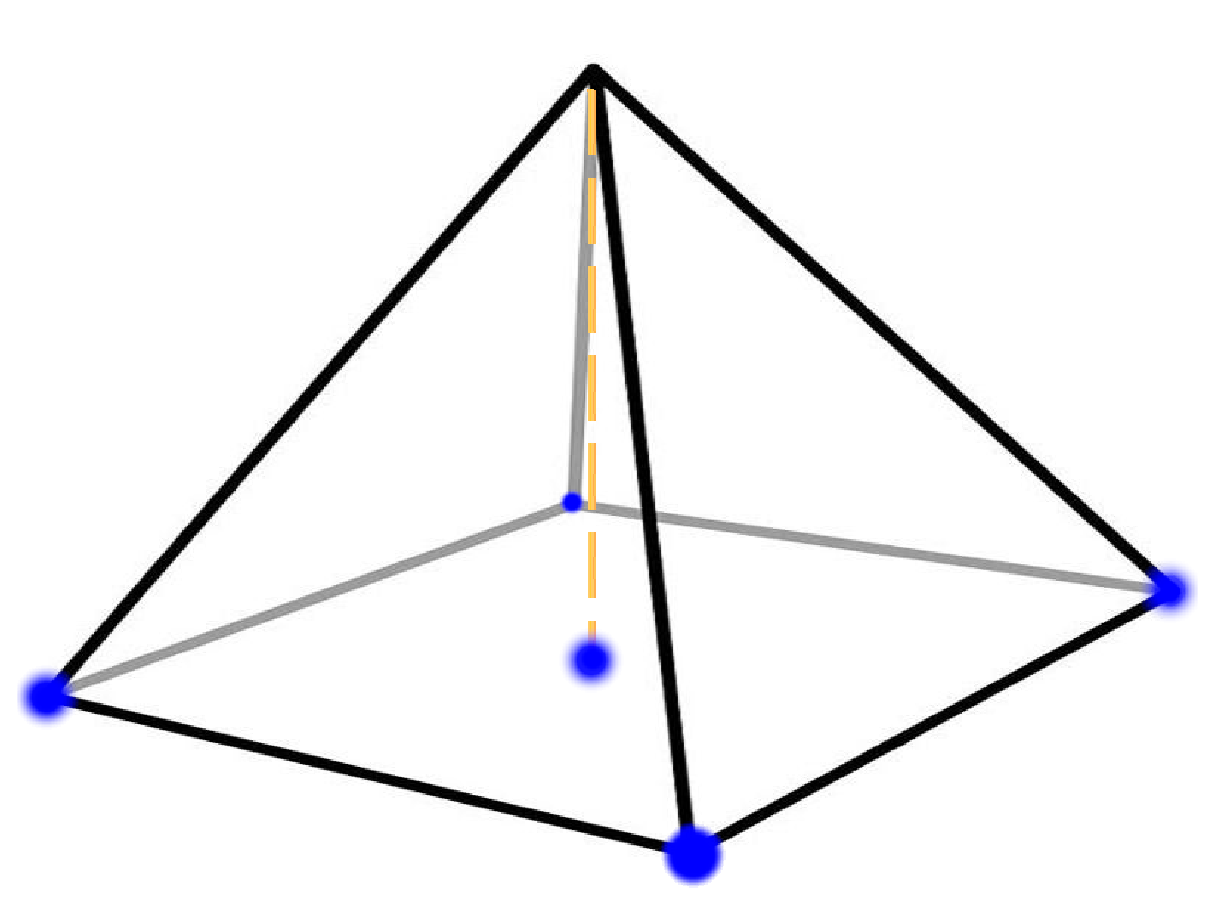
\includegraphics[width=0.5\linewidth]{figuras/piramide.eps}\\
  \caption{
Función de forma piramidal utilizada para producir las variaciones 
en el coeficiente de absorción. Esta función vale uno en un  punto dado 
y se anula en el resto de los puntos de la grilla discreta.}
 \label{fig:piramid}
\end{figure}
 La función piramidal discretizada es aproximada como un producto 
 de deltas de Kronecker $\delta a_{\ell_1,\ell_2}=\delta_{r,\ell_1}\times\delta_{s,\ell_2}$.
 Llamando $\nabla_a g(\x_{\ell_1,\ell_2})$ al valor del gradiente funcional 
 en la dirección $\delta a_{\ell_1,\ell_2}$, la versión discreta 
 de la Ecuación~\eqref{gradient_fin} resulta
\begin{equation}
\begin{aligned}
\nabla_a g(\x_{\ell_1,\ell_2}) & =- \int_0^T \int_{\Omega} \int_{S^1} \lambda(\x,\hth,t) \, \delta
  a(\x) \, u(\x,\hth,t) \, d \theta \, d\x \, dt \\ & \sim -\sum_{m,j}  \lambda_{\ell_1,\ell_2,m,j}u_{\ell_1,\ell_2,m,j} \Delta \theta \, \Delta x \, \Delta y \, \Delta t,
\end{aligned}
\label{eq:FDwin22}
\end{equation}
donde $\lambda_{\ell_1,\ell_2,m,j}\sim
\lambda(\x_{\ell_1,\ell_2},\hth_m,t_j)$ y 
$u_{\ell_1,\ell_2,m,j} \sim u(\x_{\ell_1,\ell_2},\hth_m,t_j)$. 
Cabe notar que la Ecuación~\eqref{eq:FDwin22} representa 
la derivada funcional para una única dirección $\delta a_{\ell_1,\ell_2}$ 
correspondiente a la componente $(\ell_1,\ell_2)$ del gradiente funcional discreto, 
donde el gradiente total discretizado estará dado por las perturbaciones en todas las direcciones posibles
\begin{equation}
\nabla_a g(\x)  = \left( \nabla_a g(\x_{1,1}), \nabla_a g(\x_{1,2}), \ldots, \nabla_a g(\x_{N_x+1,N_y+1})   \right).
\label{eq:grad_total}
\end{equation}
En el método adjunto, la evaluación de la Ecuación~\eqref{eq:FDwin22} 
para todas las componentes $(\ell_1,\ell_2)$ del gradiente funcional requiere 
únicamente la resolución de un problema directo de transporte, y de 
su correspondiente problema adjunto para cada fuente  generalizada $q=q_i$. 
En cambio, el método de diferencias finitas hace uso de la Ecuación~\eqref{eq:ObjFD}, que demanda la resolución de 
un número mucho más grande de problemas directos. En este último caso  deben evaluarse $(N_x+1) \times (N_y+1)$ problemas de transporte (uno por cada perturbación del coeficiente $a(\x)$ en el dominio discretizado). En el ejemplo que estamos analizando en esta sección $N_x=N_y=200$ por lo cual 
el método adjunto reduce el tiempo computacional 
en un factor $40401$.
Cabe mencionar también que el método adjunto requiere el almacenamiento 
en memoria de las soluciones completas de los problemas directos y adjunto de transporte 
para varios pasos temporales~\eqref{eq:FDwin22}. 
El algoritmo paralelo propuesto en esta Tesis es apropiado para este problema, ya que no solo permite 
reducir el tiempo computacional, si no que también distribuye los requerimientos de memoria en los diferentes nodos. 
 
Como ilustración, en la Figura~\ref{fig:gradient} se muestra 
el gradiente completo $\nabla_a g(\x_{\ell_1,\ell_2})$ para 
$1\leq \ell_1\leq N_x+1$ y $1\leq \ell_2\leq N_y+1$. 
El problema a simular consiste en una única fuente ubicada en $\x_s=(1.5,0)$ cm y un único detector ubicado en $\x_d=(0,1.0)$ cm. 
Elegimos el caso en el cual el detector mide $\tilde G_{j,i}(t)=1$.
\begin{figure}[h!]
\centering
  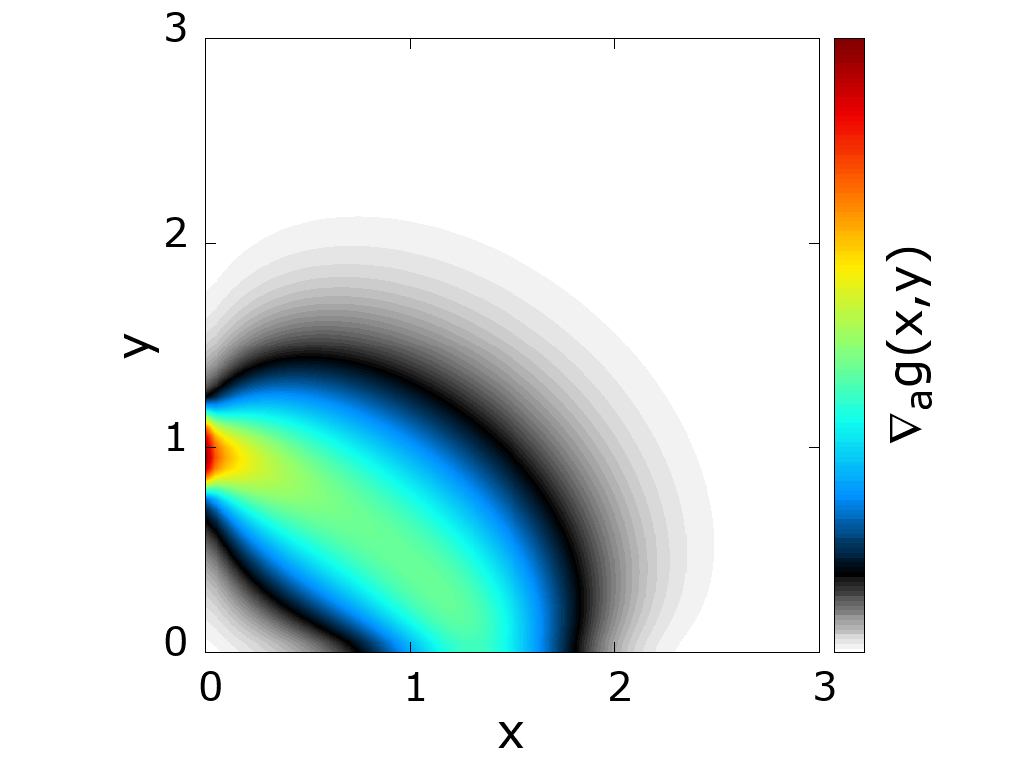
\includegraphics[width=0.5\linewidth]{figuras/gradient.png}
  \caption{
  Gradiente espacial~\eqref{eq:FDwin22} para todas 
  las direcciones discretas posibles $1\leq \ell_1\leq N_x+1$ y $1\leq \ell_2\leq N_y+1$, 
  con una única fuente y un único detector ubicados en $\x_s=(1.5,0)$ cm
  y $\x_d=(0,1.0)$ cm respectivamente. Dado que se utilizaron 
  datos artificiales, la escala carece de sentido en esta figura, 
  y por eso no se muestra.}
 \label{fig:gradient}
\end{figure} 
Como se observa en la figura, 
el gradiente contiene información de los trayectos determinados por los fotones que salen desde la fuente y arriban al detector. Dichos trayectos definen una región donde el gradiente es más 
sensible a las variaciones del medio participante. Esto muestra la importancia de contar con varias fuentes y varios detectores 
que sean capaces de sensar la totalidad del dominio. 
 
\section{Datos sintéticos con fuentes láser pulsadas} 
\label{sec:sintetic} 
En esta sección simularemos escenarios que pueden ocurrir 
en tomografía óptica. A diferencia de los casos estudiados 
hasta ahora, trataremos situaciones 
con fuentes láser pulsadas que inciden sobre la superficie del dominio. 
Modelamos la radiación colimada de las fuentes por medio 
de una función de la variable $\hth$, que tienen máximos abruptos en las direcciones incidentes de cada láser. 
Resolvemos el problema directo~\eqref{eq:RTE} con condiciones 
de borde de Fresnel, utilizando el método FC--DOM. 

Asumimos un medio con parámetros ópticos constantes $a(\x)=0.1$ cm$^{-1}$, $b(\x)=20$ cm$^{-1}$, $g=0.8$, 
$n_{\Omega}=1.4$ y $n_0=1.0$, en un dominio espacial $\Omega=[x_{\text{min}},x_{\text{max}}]\times[y_{\text{min}},y_{\text{max}}]=[0,3]\times[0,3]$ cm$^2$. 

Como primer caso supondremos una única fuente, 
centrada en $\x_{1,1}=(1.5,0)$ cm, apuntando en la dirección 
normal a la superficie, con $\theta_{1,1}=\pi/2$, y $\sigma_{\theta}=\pi/4$. 
Este láser inyecta un pulso de $60$ ps de duración. La Figura~\ref{fig:photonflux} muestra la evolución 
temporal de una ``onda de flujo de fotones'' difusos.
\begin{figure*}[h!]
\centering
  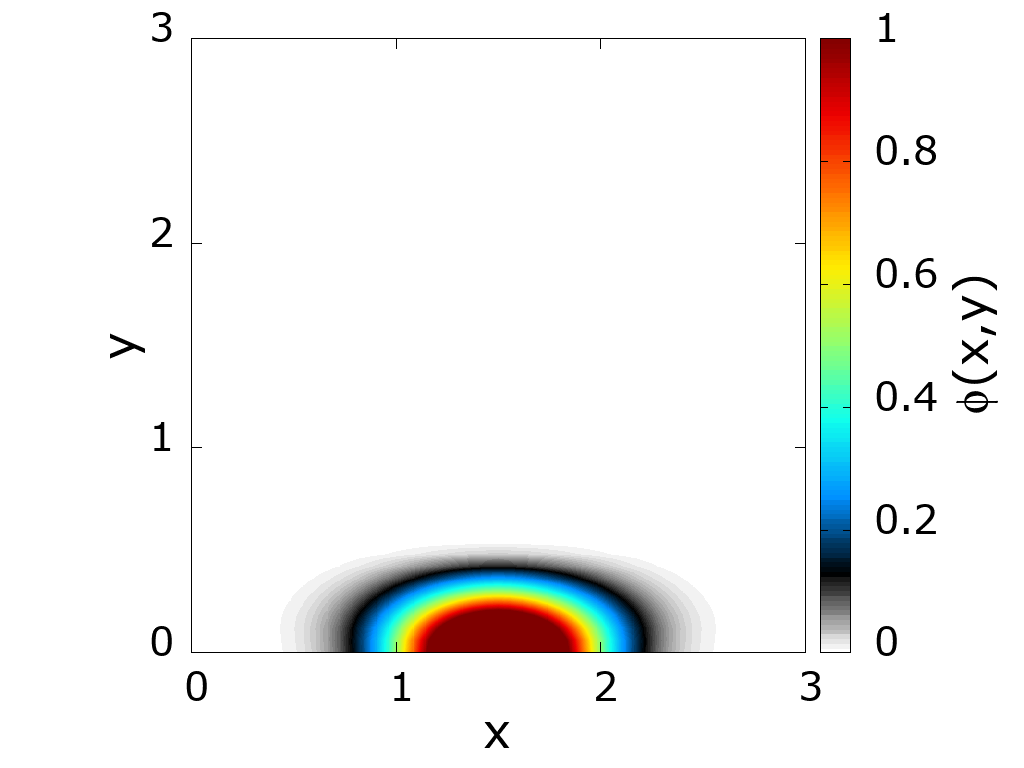
\includegraphics[width=0.325\textwidth]{figuras/sim_MB_t30.png}
  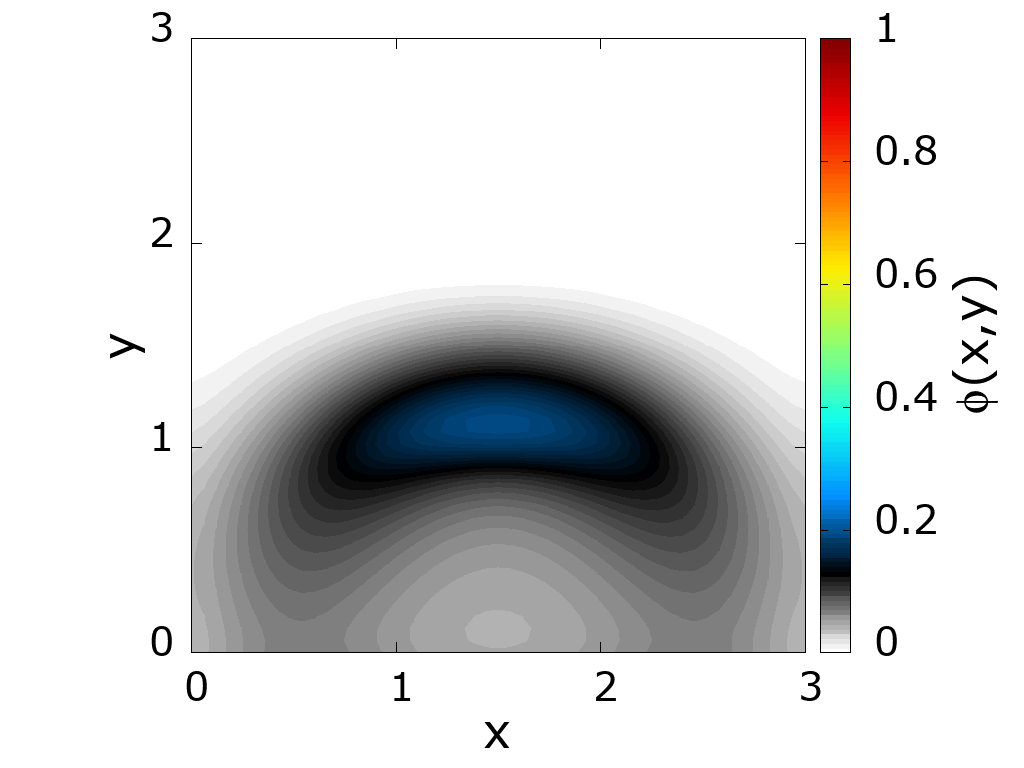
\includegraphics[width=0.325\textwidth]{figuras/sim_MB_t100.png}
  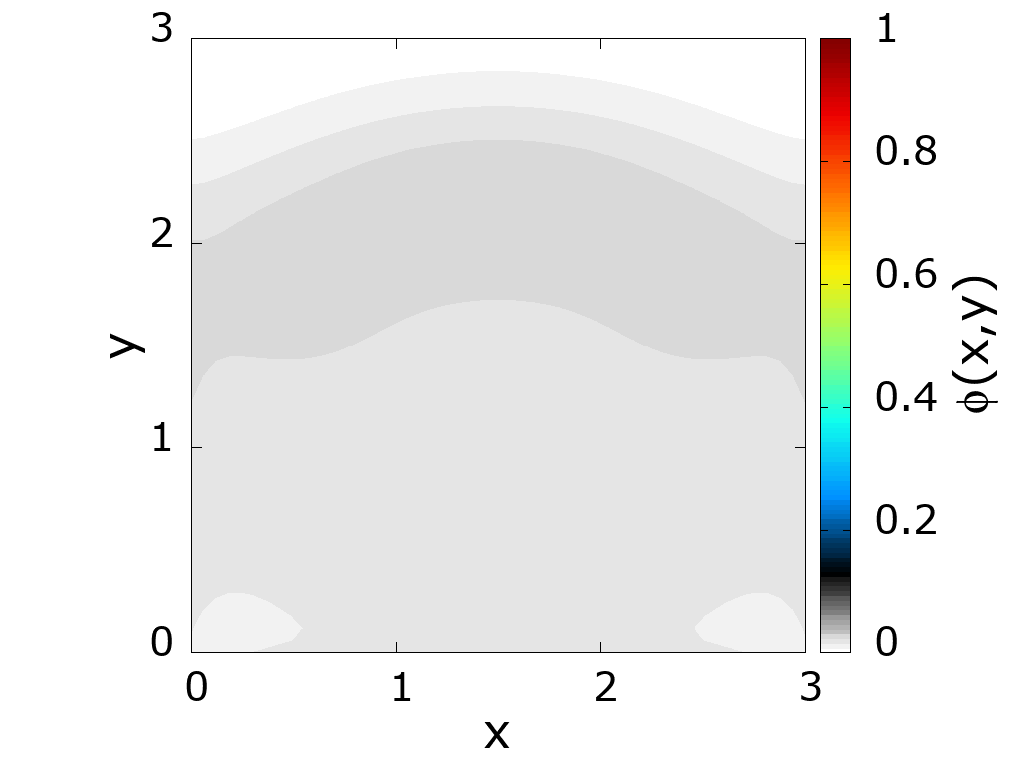
\includegraphics[width=0.325\textwidth]{figuras/sim_MB_t170.png}
  \caption{Simulación para el modelo directo utilizando 
  el método FC--DOM en paralelo. En la figura se muestra el 
  flujo escalar $\phi(\x,t)$ debido a una fuente láser 
  ubicada en $\x_s=(1.5,0)$ cm para tres tiempos diferentes. De 
  izquierda a derecha: $t=30$ ps, 
$t=100$ ps y $t=170$ ps.}
 \label{fig:photonflux}
\end{figure*}
En la Fig.~\ref{fig:detread} se muestra la lectura la lectura de un detector ubicado en 
$\x_d=(0.0,0.75)$ cm en función del tiempo. 
Dado que en situaciones realistas se espera 
que los datos experimentales presenten ruido, agregamos un 10\% de fluctuaciones aleatorias. 
Este tipo de simulaciones se utiliza para construir datos sintéticos 
en el método MB.
\begin{figure}[h!]
\centering
  \includegraphics[width=0.48\linewidth]{figuras/detread_sweep.eps}
  \caption{Lectura del detector ubicado en $\x_d=(0.0,0.75)$ cm para 
  una única fuente (curva roja). Agregando un 10\% de ruido aleatorio 
 se obtiene la señal sintética (curva negra).}
 \label{fig:detread}
\end{figure}

A continuación resolveremos un problema directo en el cual 
se introducen diversas fuentes pulsadas que se encienden en distintos tiempos. 
Mostramos la resolución de este tipo de problemas, ya que constituye 
una simulación típica utilizada en la estrategia FMS. 
En este ejemplo se inyecta radiación en la dirección normal a 
la superficie por cuatro láseres ubicados en el centro de las caras. 
Cada uno de estos pulsos tiene una duración de $60$ ps, 
y se encienden con una separación temporal de $\tau=200$ps. 
El orden de encendido es: primero la fuente ubicada en $y_{\text{min}}$, seguida de la fuente 
en $y_{\text{max}}$, luego la ubicada en $x_{\text{min}}$ y finalmente 
se enciende la fuente en $x_{\text{max}}$.   
En la resolución que utiliza el método FMS estas cuatro fuentes 
constituyen una única fuente generalizada ($N_q=1$ y $N_s=4$). 
Se imponen estos retardos temporales 
para desacoplar las señales 
originadas por las fuentes individuales proveniente de diferentes lugares.
La Figura~\ref{fig:photonflux2} muestra el flujo escalar resultante 
para distintos tiempos.
 
\begin{figure*}[h!]
\centering
  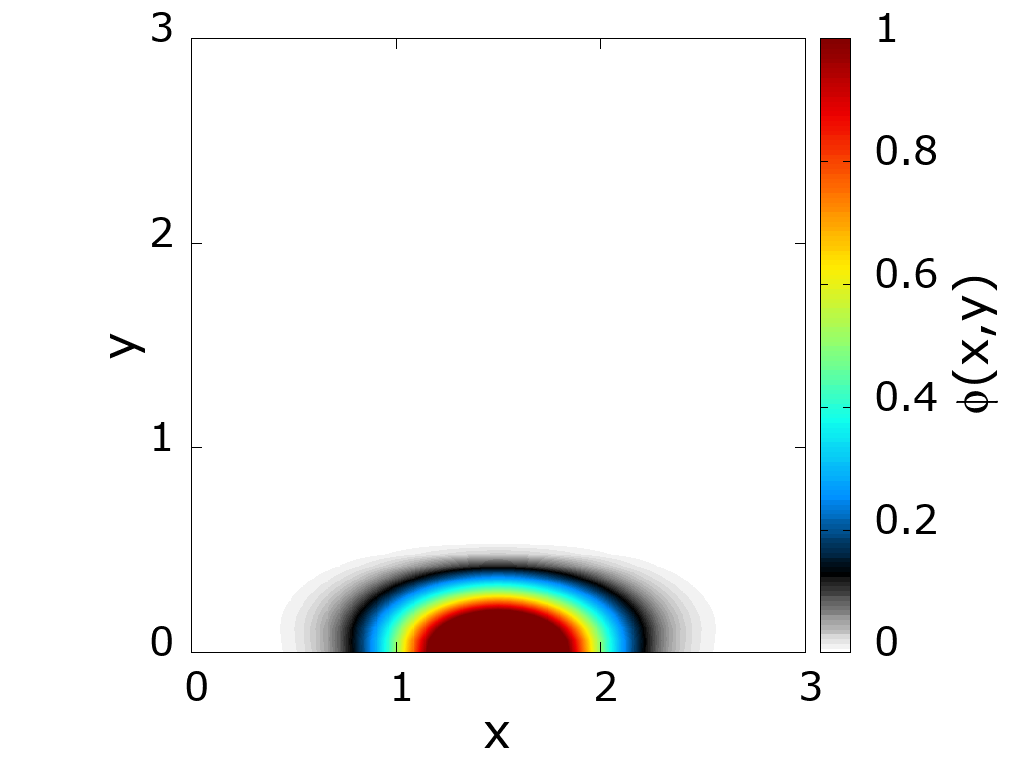
\includegraphics[width=0.325\textwidth]{figuras/sim_FMS_t30.png}
  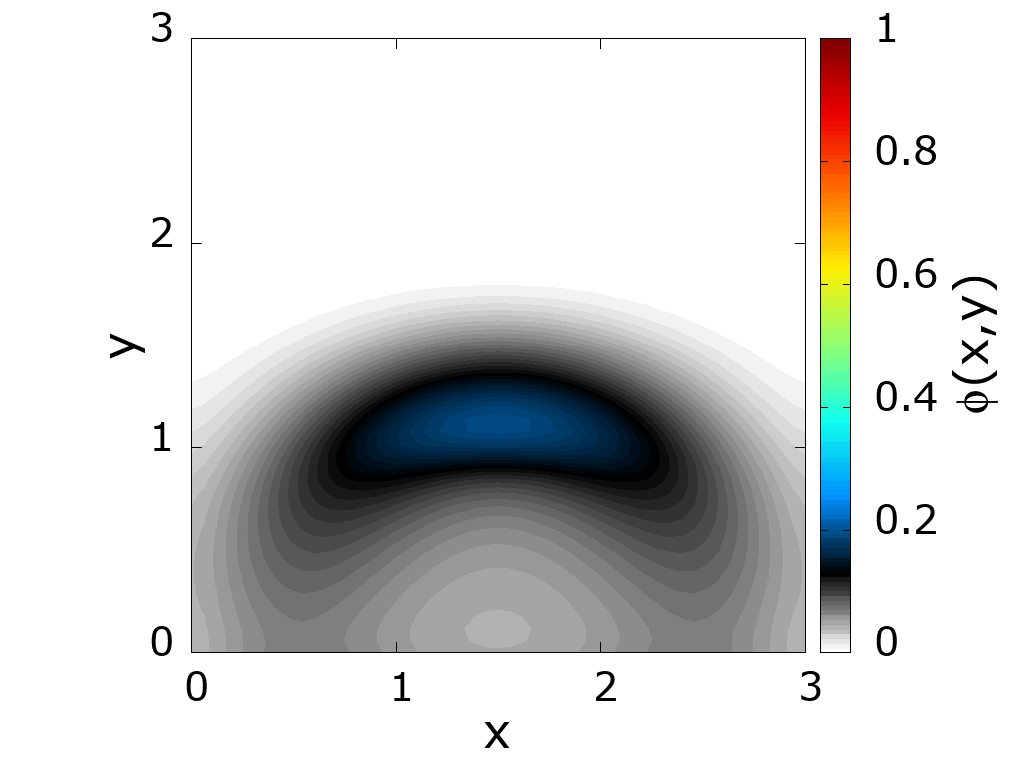
\includegraphics[width=0.325\textwidth]{figuras/sim_FMS_t100.png}
  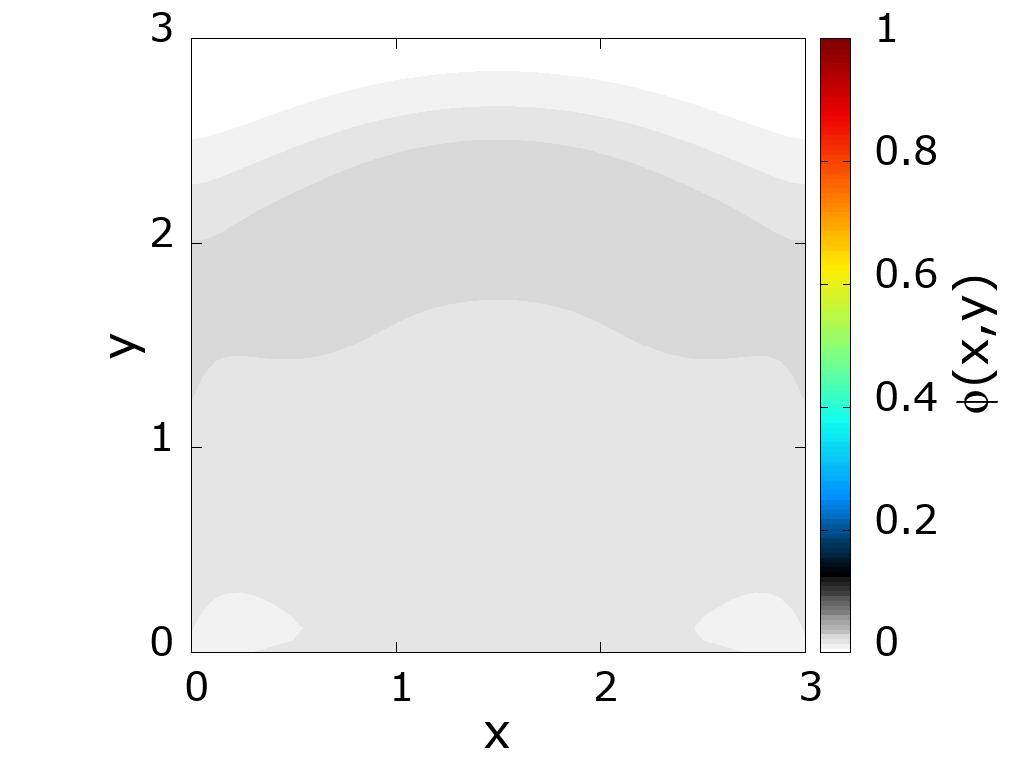
\includegraphics[width=0.325\textwidth]{figuras/sim_FMS_t170.png}\\
  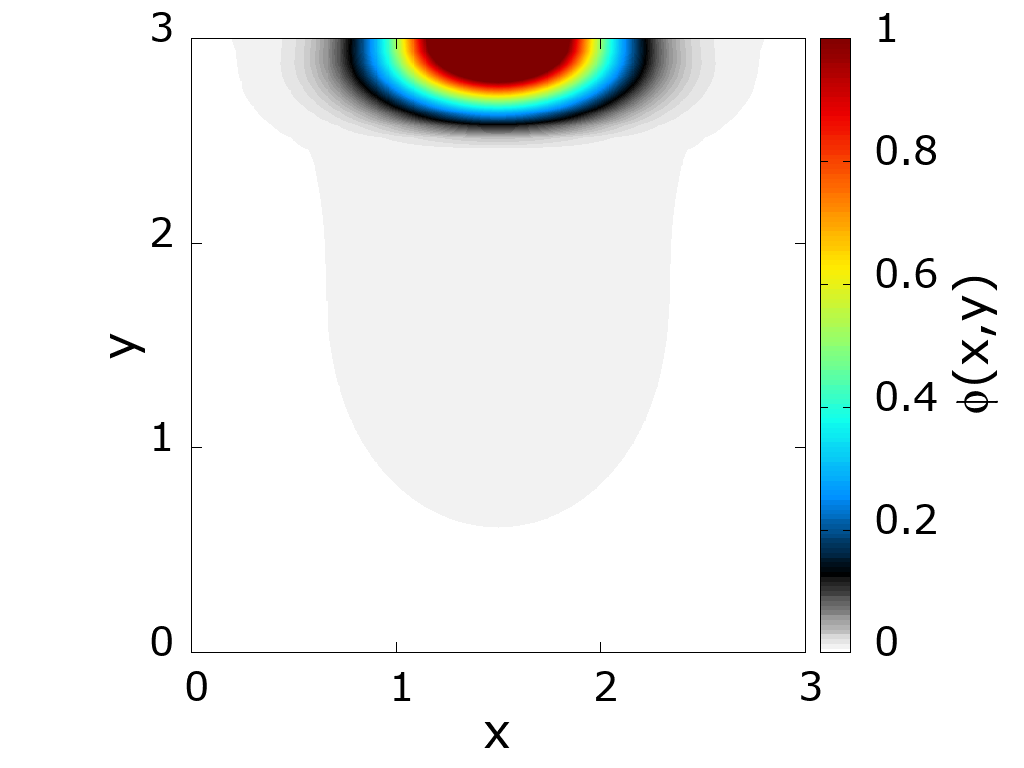
\includegraphics[width=0.325\textwidth]{figuras/sim_FMS_t230.png}
  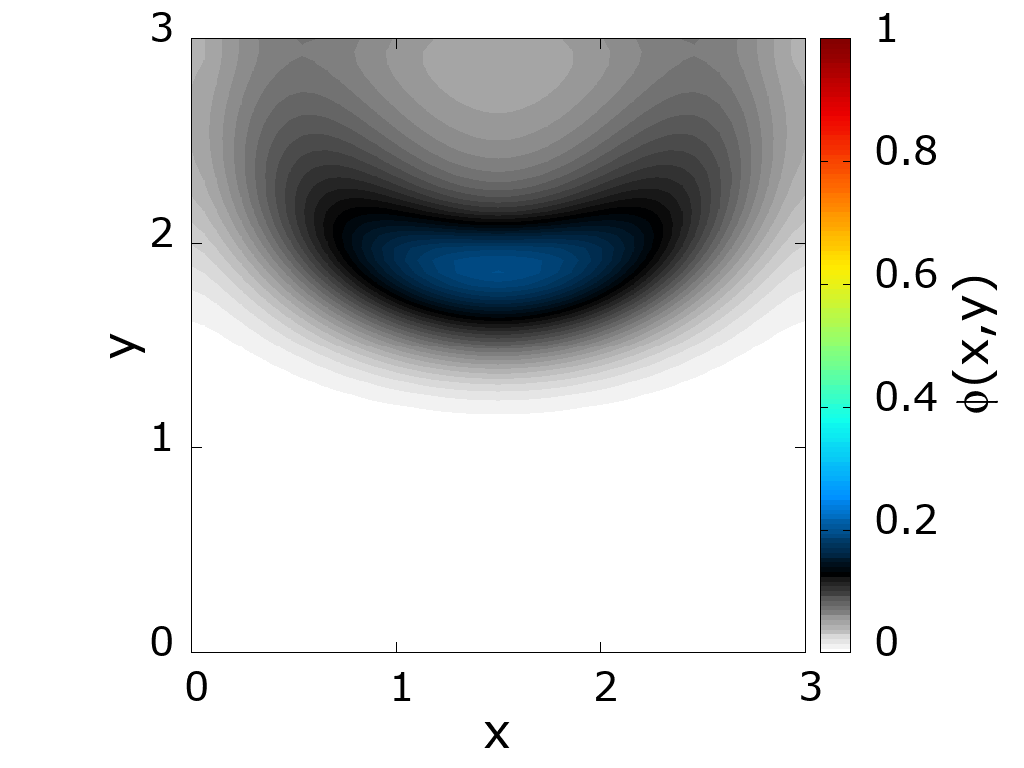
\includegraphics[width=0.325\textwidth]{figuras/sim_FMS_t300.png}
  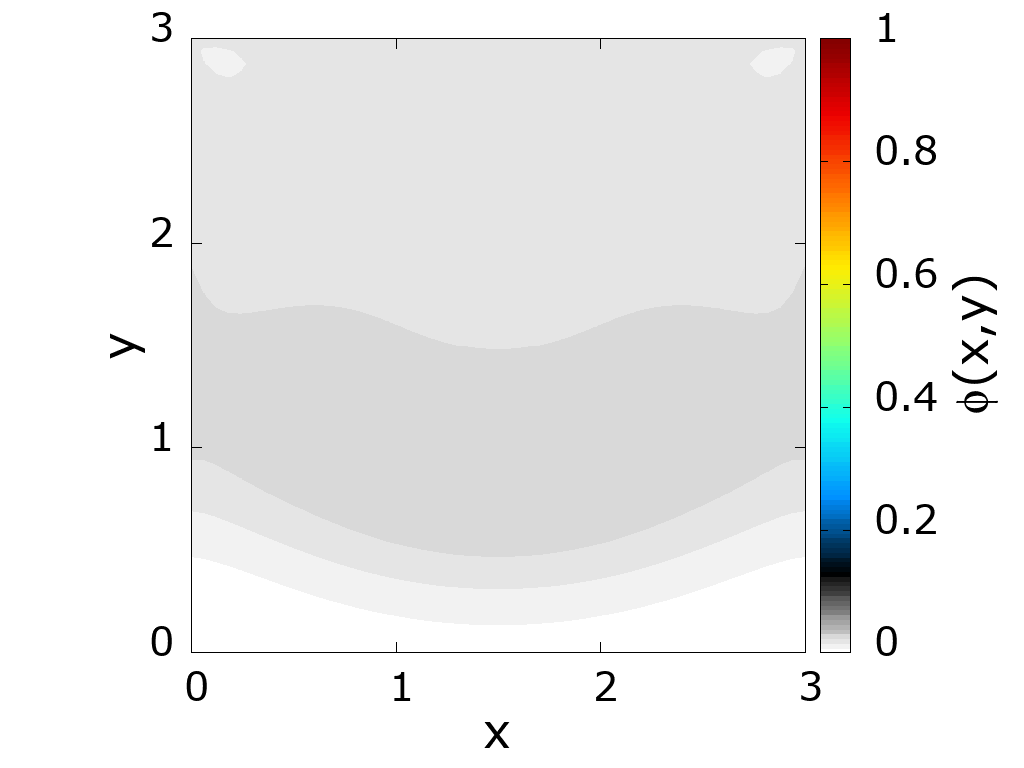
\includegraphics[width=0.325\textwidth]{figuras/sim_FMS_t370.png}\\
  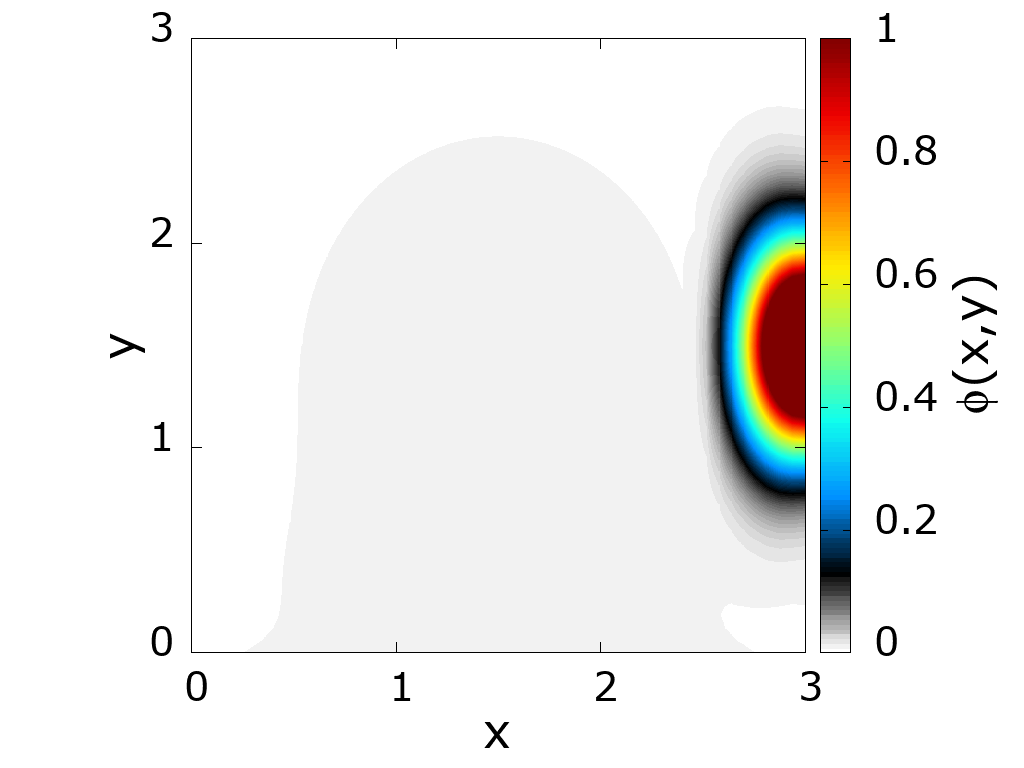
\includegraphics[width=0.325\textwidth]{figuras/sim_FMS_t430.png}
  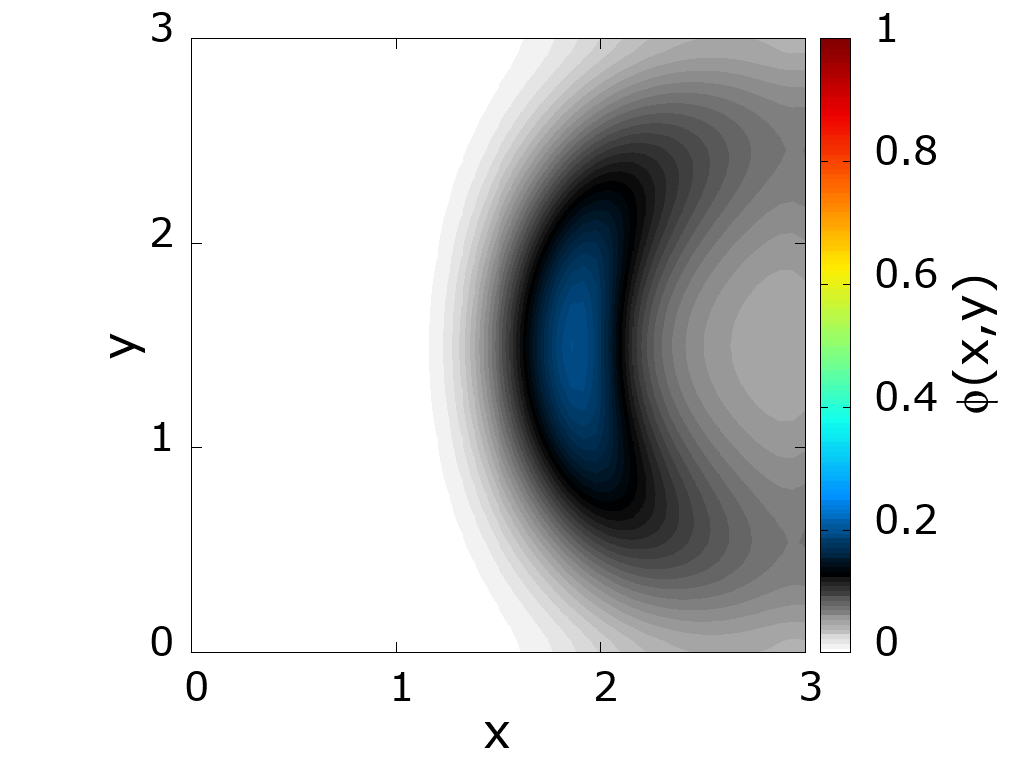
\includegraphics[width=0.325\textwidth]{figuras/sim_FMS_t500.png}
  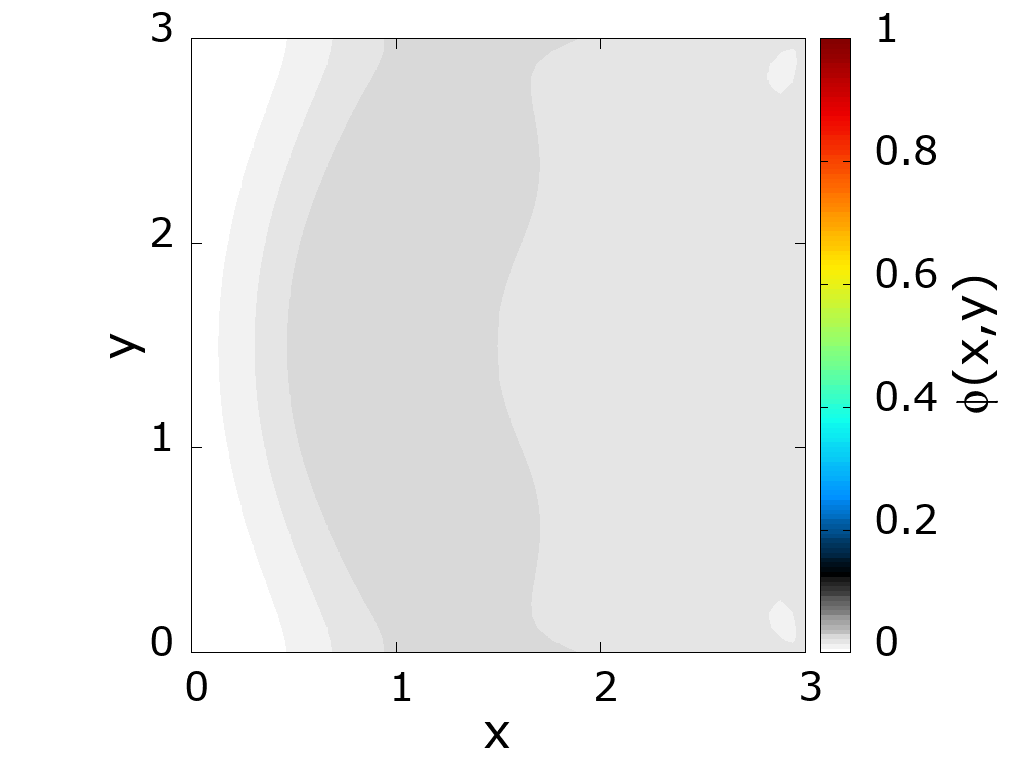
\includegraphics[width=0.325\textwidth]{figuras/sim_FMS_t570.png}\\
  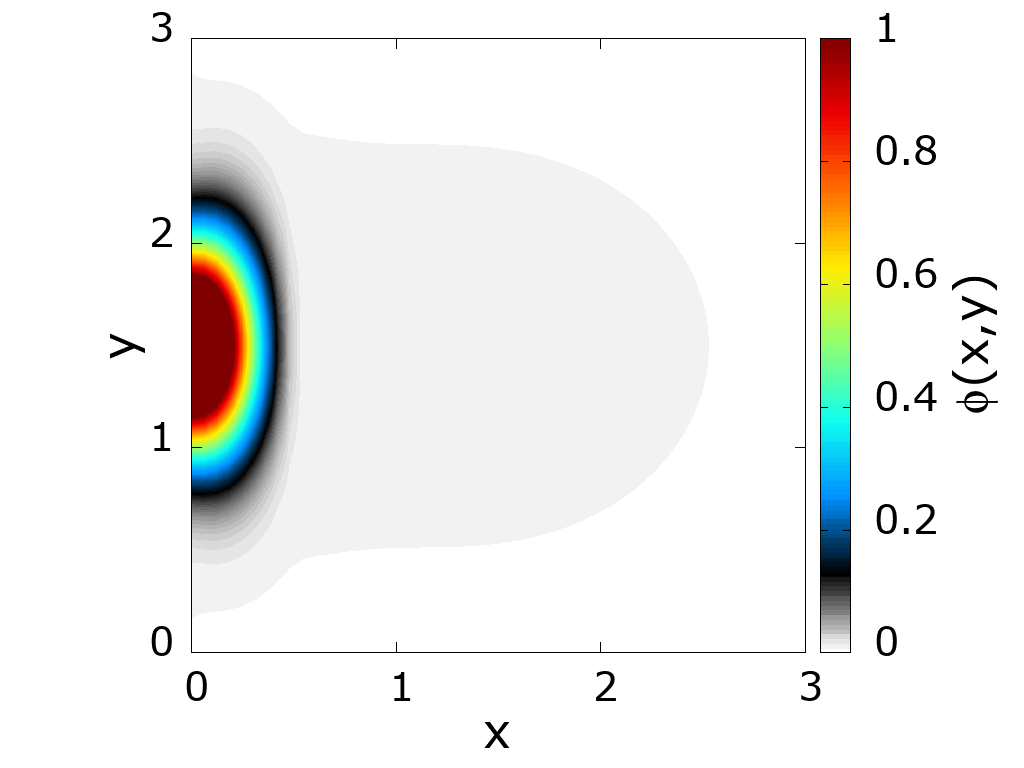
\includegraphics[width=0.325\textwidth]{figuras/sim_FMS_t630.png}
  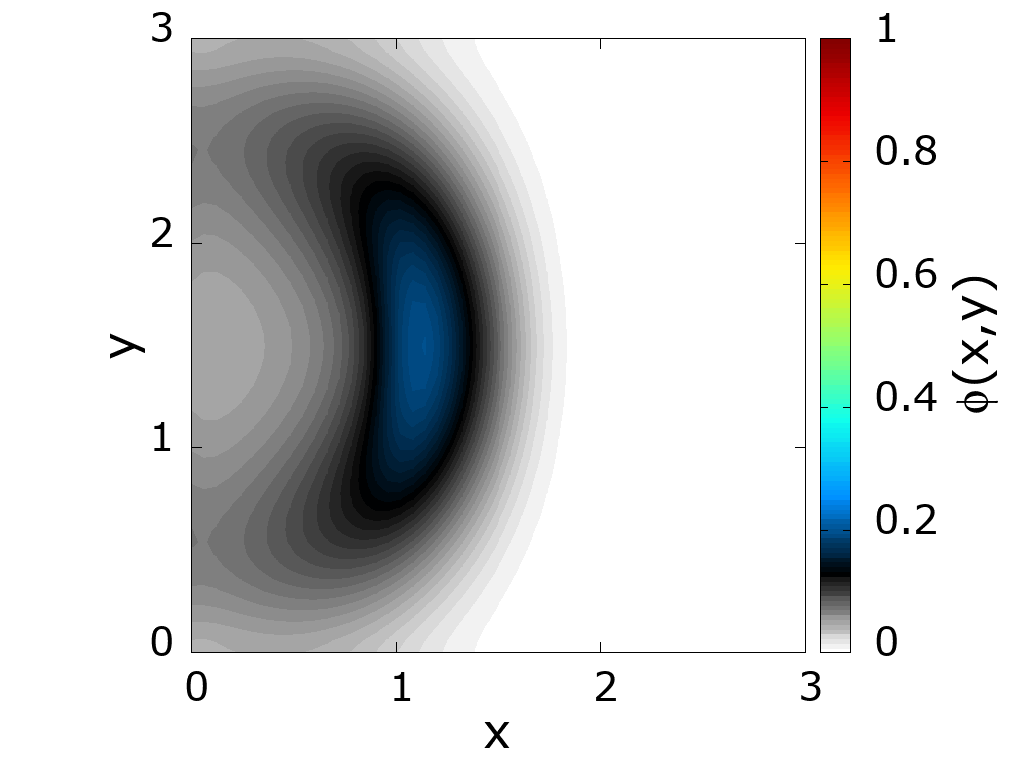
\includegraphics[width=0.325\textwidth]{figuras/sim_FMS_t700.png}
  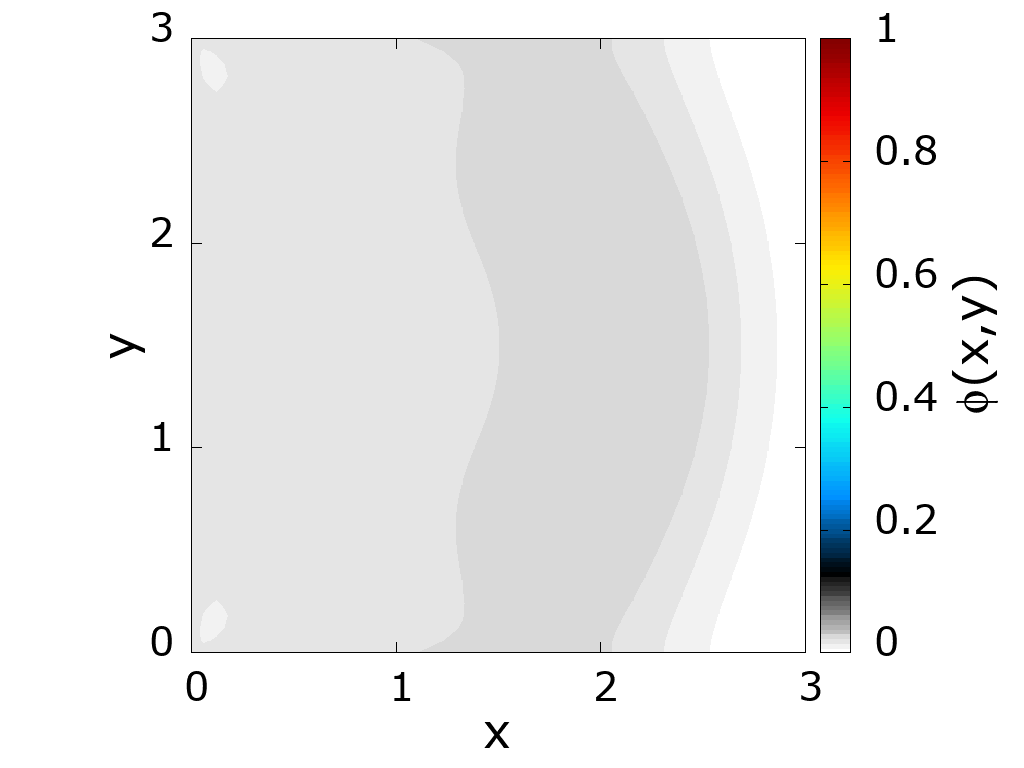
\includegraphics[width=0.325\textwidth]{figuras/sim_FMS_t770.png}
  \caption{Simulación para el problema directo utilizando 
  el método FC--DOM en paralelo y asumiendo una única fuente 
  generalizada que contiene cuatro fuentes láser que se encienden 
  a distintos tiempos. De 
  izquierda a derecha y de arriba hacía abajo: $t=30$ ps, $t=100$ ps y $t=170$ ps, 
   $t=230$ ps, $t=300$ ps y $t=370$ ps,  $t=430$ ps, $t=500$ ps y $t=570$ ps, 
    $t=630$ ps, $t=700$ ps y $t=770$ ps.}
 \label{fig:photonflux2}
\end{figure*}

La Figura~\ref{fig:detread2} muestra los valores que mide un 
detector ubicado en $\x_d=(3.0,2.25)$ en distintos tiempos. 
Como puede observarse, las señales producidas por cada fuente 
se superponen. Esto contrasta con la estrategia MB, 
donde la información de cada fuente está desacoplada del resto.  

\begin{figure}[h!]
\centering
  \includegraphics[width=0.48\linewidth]{figuras/detread_prop.eps}
  \caption{Lectura del detector ubicado en $\x_d=(3.0,2.25)$ para las cuatro fuentes superpuestas, en función del tiempo 
  (curva roja). Agregando un 10\% de ruido aleatorio 
 se obtiene la señal sintética (curva negra).}
 \label{fig:detread2}
\end{figure}

\section{Algoritmo para la resolución de problemas inversos}
\label{sec:inversesolv}

Como se indicó anteriormente, proponemos en esta Tesis para la utilización de un algoritmo novedoso para el tratamiento de  
problemas inversos. Esta estrategia se basa en el uso 
de multiples fuentes escalonadas en el tiempo (FMS), 
en lugar de la estrategia de barrido (MB) que subyace 
en los métodos tradicionalmente presentados en la literatura. 
En estos métodos previos,  por cada fuente láser deben realizarse simulaciones separadas para el par de problemas directo--adjunto, y luego combinar los resultados para obtener el gradiente utilizado en el método de minimización.
 Por el contrario, en el método FMS que proponemos en nuestro trabajo,
se construye la función objetivo utilizado una única fuente 
generalizada que contiene a todas las fuentes láser, de forma tal 
que se utiliza {\em una única simulacion del par directo--adjunto}. Como se demuestra en la sección~\ref{sec:inverseres} 
(de manera cualitativa en las Figuras~\ref{fig:itdet} y~\ref{fig:ithead} 
y de forma cuantitativa en las Figuras~\ref{fig:reconst} y~\ref{fig:rechead}), nuestro método  
reduce los tiempos de cómputo de manera significativa 
(\eg en un factor de seis), sin que se 
produzca ningún deterioro en la calidad de la imagen obtenida. 

Resolvemos los problemas inversos basandonos en el método 
iterativo cuasi--Newton de descenso de gradiente lm--BFGS. 
En detalle, este método busca el coeficiente de absorción que minimiza la Ec.~\eqref{eq:FObjpr}  
sujeto a las restricciones $a^l(\x) \leq a(\x) \leq a^u(\x) ~\forall \x$, o sea, buscamos 
el coeficiente de absorción $a(\x)$ dado por 
\begin{equation}
\begin{split}
\begin{aligned}
a(\x)=\text{argmin}_{a^l \leq \widetilde a(\x) \leq a^u} \Lambda[a].
\end{aligned}
\end{split}
\label{eq:minprob}
\end{equation}
Las restricciones de los valores admisibles de la función 
$\widetilde a(\x)$ es un conocimiento previo dado por las  propiedades de absorción generales del medio considerado. Una propiedad física que siempre debe cumplirse es que   
$a^l(\x)\ge 0$. Información adicional adquirida por 
técnicas de imagenes 
puede incorporarse para reducir el espacio de soluciones admisibles. 

El algoritmo para la resolución del problema inverso~\ref{algfcinv},
procede de la siguiente manera. A partir de una estimación inicial $a^0(\x)$ para el
coeficiente de absorción y utilizando las lecturas de los detectores experimentales
$\widetilde{G}_{j,i}$, con $j=1, \ldots,N_d$ y $i=1,\ldots,N_q$, se resuelven
los problemas directos y adjuntos~\eqref{eq:RTE}
y~\eqref{eq:AdjointProblem}, y se calcula el gradiente 
funcional~\eqref{eq:FDwin22}. Seguidamente, este gradiente 
se utiliza en el algoritmo lm--BFGS, que devuelve una actualización para 
coeficiente de absorción $a^1(\x)$ el cual reduce las diferencias entre
las lecturas de los detectores experimentales y los valores para los detectores simulados.
La iteración de este procedimiento converge, mediante el método lm-BFGS, al mínimo 
de la función objetivo~\eqref{eq:FObjpr}.

El pseudocódigo con el cual solucionamos el problema inverso de transporte radiativo, 
para un dado número de iteraciones $i_{\text{max}}$, se presenta en 
Algoritmo~\ref{algfcinv}. Aquí $C \in \mathbb{R}$ representa un criterio 
de convergencia preestablecido. El algoritmo se itera mientras el valor 
de la función objetivo esté por encima de dicho criterio de convergencia.
\begin{algorithm}
\caption{Pseudocódigo para la resolución del problema inverso}
\label{algfcinv}
\begin{algorithmic}[1]
\State Dar una estimación inicial $a^0(\x)$
\State \textbf{para} $i=1,\ldots,i_{\text{max}}$ \textbf{hacer}
\State \hskip0.5em \textbf{para} cada fuente generalizada $q_j, j = 1,\ldots,N_q$ \textbf{hacer}
\State \hskip0.75em Resolver el problema directo por medio del Algoritmo~\ref{algfc}
\State \hskip0.75em Evaluar ec.~\eqref{eq:FObjpr}, si $ \Lambda[a] < C $ ir a \ref{al:end}.
\State \hskip0.75em Resolver el problema adjunto mediante el Algoritmo~\ref{algfc}
\State \hskip0.5em\textbf{terminar}
\State \hskip0.5em Construir el gradiente ec.~\eqref{eq:FDwin22}
\State \hskip0.5em Llamar al algoritmo lm-BFGS para actualizar el coeficiente $a^{i+1}(\x)$.       
\State \label{al:end} \textbf{terminar} con $a(\x)=a^i(\x)$
\end{algorithmic}
\end{algorithm}


\section{Reconstrucciones numéricas del problema inverso}
\label{sec:inverseres}
En esta sección demostraremos las notables 
ventajas que se obtienen utilizando nuestros métodos 
aplicandolos a la solución de dos problemas de sumo 
interés en tomografía óptica y diagnostico médico: 
1) Imagen de tejidos cancerosos en un cuello humano; 
2) Respuesta hemodinámica en un modelo de cabeza humana.
En ambos, los problemas inversos de tomografía óptica que consideramos 
conciernen configuraciones en las cuales se buscan inclusiones 
sobre un tejido de ``fondo'' que se asume conocido. 
Estas inclusiones están caracterizadas por un índice 
de absorción que la del tejido que la rodea. Los excesos en la absorción son originados 
por el aumento de la hemoglobina oxigenada. 
Este aumento se puede producir por la presencia de un tumor (angiogénesis tumoral) en el tejido 
(de gran importancia en diagnósticos médicos~\cite{Althobaiti2017,Guven2003,Zhu2005,Zhu2010,Fujii2016b}).
El exceso de hemoglobina oxigenada también puede dispararse por la respuesta hemodinámica debido a la activación 
de una región determinada del cerebro (de interés 
en neurociencias~\cite{Boas2001,bluestone2001,Arridge1999,Hernandez2020}).

Resolvemos el problema inverso sobre la base de los datos sintéticos 
que se obtienen de la solución numérica del problema directo para 
un coeficiente de absorción ``buscado'', $a^v(\x)$. 
Como se describió en la sección anterior, agregamos un 10\% de ruido 
aleatorio a las lecturas resultantes de los detectores para tener en cuenta el ruido experimental. 
Estudiaremos la convergencia por iteración del algoritmo~\ref{algfcinv} 
para un número variable de fuentes y detectores, para una  configuración dada. 
Para evaluar la convergencia en el proceso de reconstrucción cuantificamos el error en la norma $L^2$ definido como
\begin{equation}
\begin{split}
\begin{aligned}
E(i)=\sqrt{\frac{\int_{\Omega}(a^v(\x)-a^i(\x))^2  d\x}{\int_{\Omega}a^v(\x) d\x}}
\end{aligned}
\end{split}
\label{eq:errl2}
\end{equation}
donde $E(i)$ corresponde al error $L^2$ para la iteración $i$, 
donde $a^v(\x)$ es el coeficiente de absorción ``verdadero'', y $a^i(\x)$ 
es el coeficiente de absorción obtenido por el algoritmo~\ref{algfcinv}.

\subsection{Imagen de tumor en cuello humano}

El primer caso de prueba concierne a la aplicación potencial 
de la técnica de tomografía óptica en el diagnóstico 
de pacientes para los cuales se dispone de imagenes por resonancia magnética (MRI)
del cuello (Fig.~\ref{fig:mriim}). 
Describimos una situación teniendo 
en mente la posible evolución de la metástasis 
en una región específica del cuerpo (el cuello), tiempo después 
de haber adquirido la imagen MRI. Similarmente, el procedimiento 
podría utilizarse para seguir la evolución del tratamiento de un tumor en esta región. 
La portabilidad y el bajo costo de los sistema de tomografía óptica 
hace que estos dispositivos sean mucho mas accesibles para el diagnóstico 
que las imágenes obtenidas por sistemas MRI, para monitorear 
la evolución del tratamiento y el avance de un tumor de forma regular. 

En las referencias~\cite{Fujii2016b,Fujii2016} se 
pueden encontrar estudios sobre el problema directo de la propagación de la luz en el cuello humano. 
Nosotros utilizamos un modelo similar, 
para el estudio del problema inverso 
correspondiente (el cual requiere la resolución 
repetida del par de problemas directo--adjunto, 
como se describe en el Algoritmo~\ref{algfcinv}).  
En particular, nos enfocaremos en la 
reconstrucción de las propiedades del medio, 
el estudio de la convergencia y los tiempos computacionales 
requeridos por los diferentes métodos. 

Buscaremos la existencia de un tumor en el tejido blando. 
 Esto se debe 
a que la angiogénesis tumoral sólo ocurre en este tipo 
de tejidos.
Tanto los coeficientes de la columna vertebral, 
como los de la médula espinal, y de la tráquea 
se mantendrán fijos en el proceso de reconstrucción (Tabla~\ref{tab:cuello}), y fueron tomados de las referencias~\cite{Bashkatov2011,Dehaes2011,Fujii2016}.
\begin{table}[h!]
\caption{Propiedades ópticas para el modelo de cuello humano}
\vspace{-0.3cm}
\begin{center}
\begin{tabular}{ccccccc}
\hline
Órgano & ~ $a[1/cm]$ & ~ & $b[1/cm]$ ~ & $g$ ~ & $n_{\Omega}$ \\
\hline
Tejido blando & ~$0.3$ & ~ & $80$ ~ &$0.9$ ~  & $1.4$ \\
Tráquea & ~$0.0$ & ~ & $0.0$ ~ &$0.0$ ~ &  $1.0$\\
Columna vertebral & ~$0.25$ & ~ & $148$ ~ &$0.9$   ~ &  $1.4$ \\
Médula espinal & ~$0.17$ & ~ & $882$ ~ &$0.9$  ~ &  $1.4$ \\
\hline
\end{tabular}
\label{tab:cuello}
\end{center}
\end{table}
Para simplificar el modelo, tomamos el coeficiente de refracción 
de la traquea cómo $n_{\Omega}=1.4$. Esto evita las dificultades 
encontradas para el modelado de la interfase entre la traquea y el tejido blando. Para mayor precisión se requiere tener en cuenta la reflexión 
de Fresnel en esta interfase geométricamente compleja. Otras simplificaciones 
adicionales utilizadas consistieron en no considerar los vasos sanguíneos, y en la geometría del cuello, que se asumió cuadrado.

Restringimos la presencia de las inclusiones (tumores) 
a regiones levemente alejadas de la superficie del cuello.  Este procedimiento permite una mejor 
convergencia en el problema de reconstrucción, y previene 
la amplificación de los errores numéricos, originados por la existencia 
de las capa límite~\cite{Gaggioli2021} discutidas en la Sección~\ref{sec:blayer}. En consecuencia fijamos el valor  $a(\x)=a^0(\x)$ 
al valor del fondo en las proximidades de los bordes, para puntos a una distancia menor a $0.5$ cm.
El mínimo $a^l$ para el coeficiente de absorción vendrá dado 
por los valores del ``fondo'' del tejido analizado (que se asume conocido \textit{a priori}). 
El límite superior estará dado por valores típicos del coeficiente de absorción 
para el tejido que se está examinando, y lo fijaremos en $a^u=1$ cm$^{-1}$.

A partir de la imagen MRI se obtiene el coeficiente $a^0(\x)$ para la iniciación de las iteraciones. En nuestro 
ejemplo tomamos la imagen de la Fig.~\ref{fig:mriim}, 
de donde se obtienen los coeficientes de absorción $a^0(\x)$ y 
dispersión $b(\x)$ que se muestran en la Fig.~\ref{fig:mriimc} 
a la izquierda y derecha, respectivamente.
\begin{figure}[h!]
\centering
  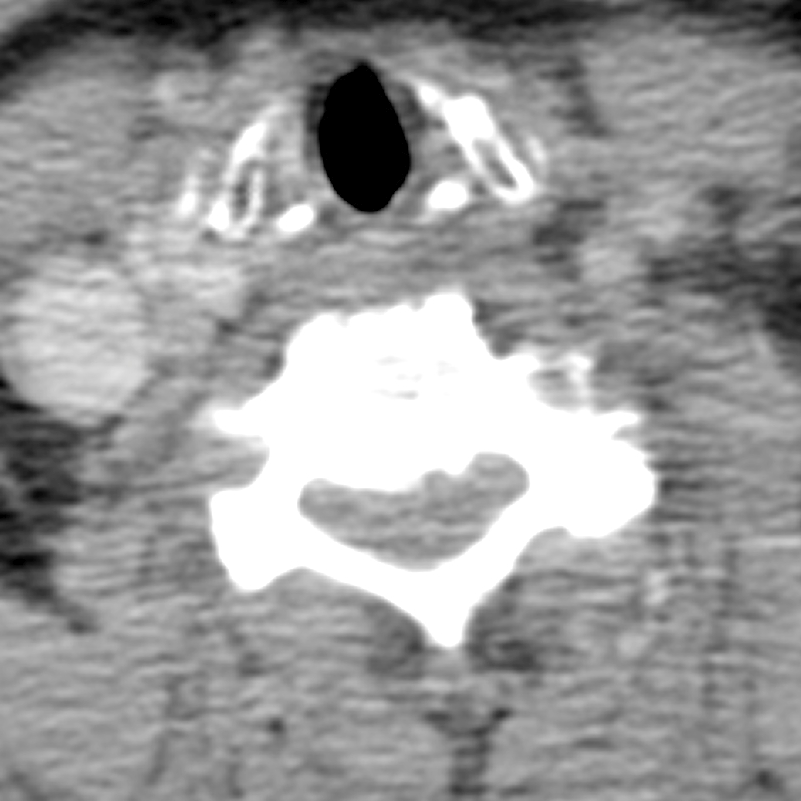
\includegraphics[width=0.25\linewidth]{figuras/neck_mri.png} 
  \caption{Imagen de Resonancia Magnética~\cite{CCommons} para el modelo de cuello humano empleado. } 
 \label{fig:mriim}
\end{figure}

\begin{figure}[h!]
\centering
  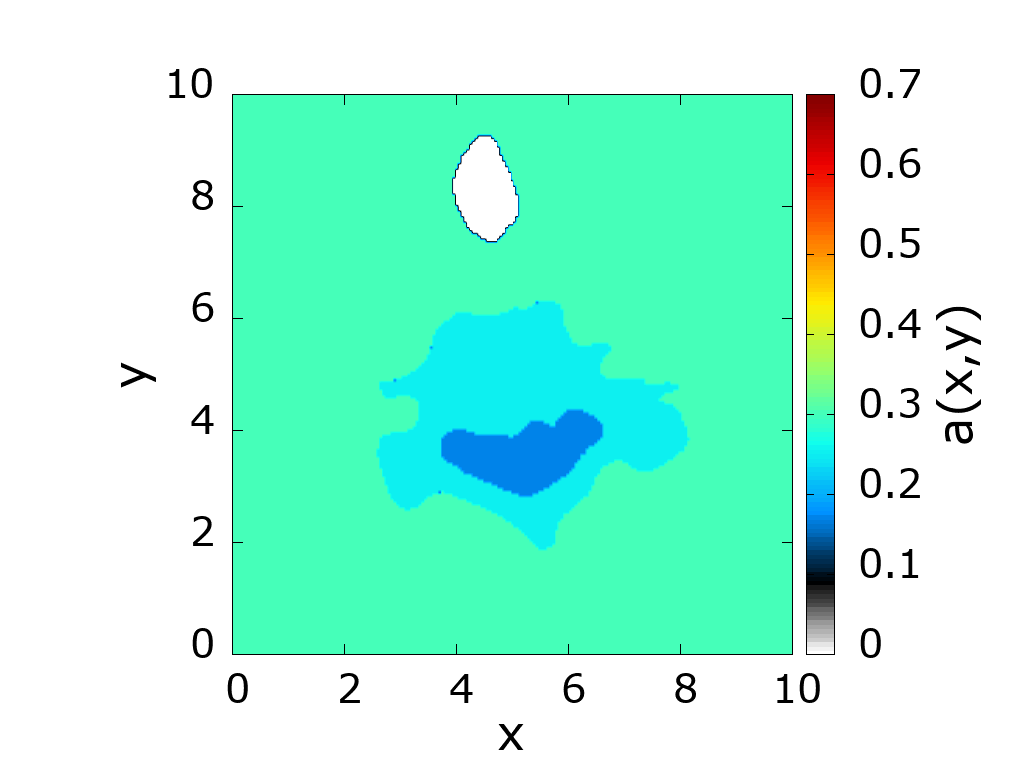
\includegraphics[width=0.48\linewidth]{figuras/neck_i.png} 
  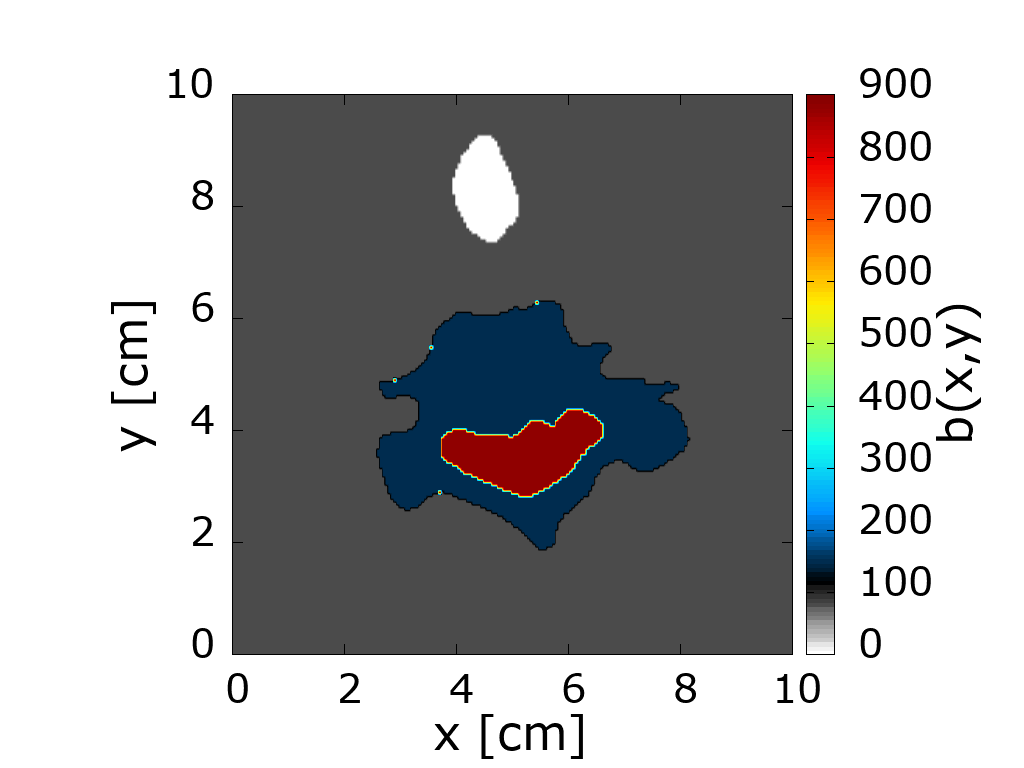
\includegraphics[width=0.48\linewidth]{figuras/neckmss_scatt.png} 
  \caption{Izquierda: coeficiente de absorción 
  generado a partir de la imagen~\ref{fig:mriim}, el cual fue utilizado como el coeficiente 
  inicial $a^0(\x)$ en las reconstrucciones del coeficiente de absorción para éste modelo. 
  Derecha: coeficiente de dispersión para el modelo de cuello humano.
  Los coeficientes de absorción y dispersión 
  para los distintos órganos fueron tomados de las referencias\cite{Bashkatov2011,Dehaes2011,Fujii2016}. } 
 \label{fig:mriimc}
\end{figure}

En esta demostración, para el método FMS empleamos una única fuente generalizada 
la cual contiene multiples fuentes láser. Las diferentes fuentes láser 
contenidas en esta única fuente generalizada iluminan el borde del dominio $\partial \Omega$ 
en la dirección normal al mismo, inyectando la radiación que atraviesa 
el medio participante, sensándolo, y luego es recolectada por los detectores. 
\begin{figure}[h!]
\centering
  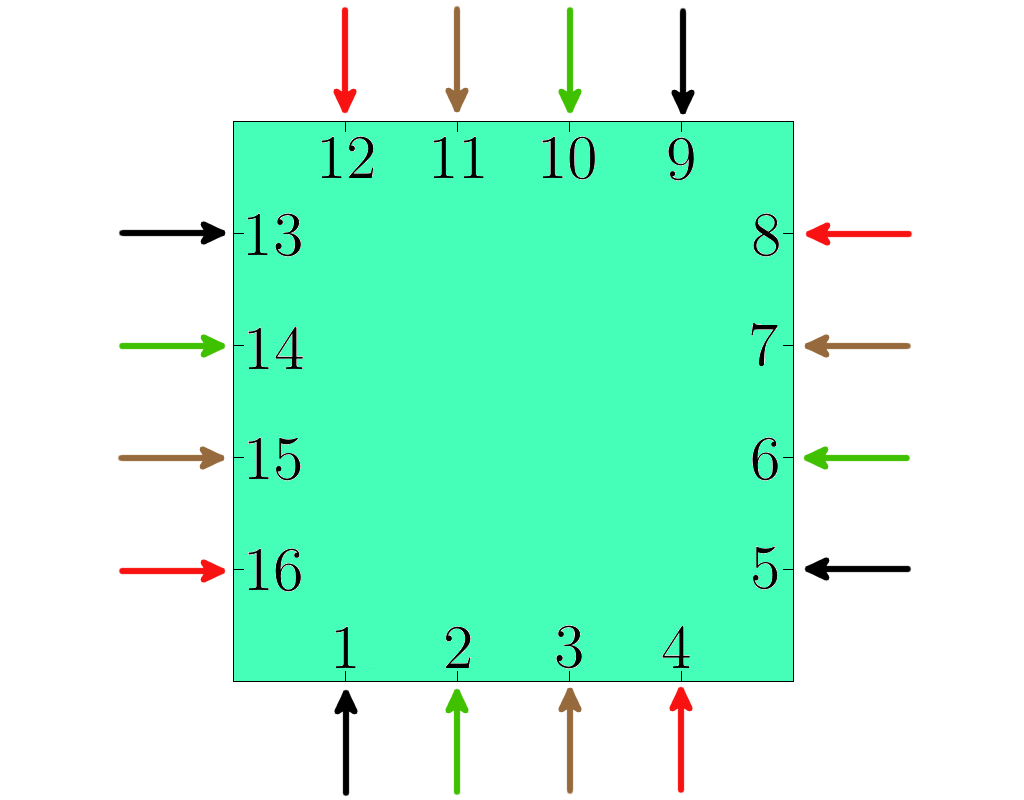
\includegraphics[width=0.48\linewidth]{figuras/neck_srcs.png}
  \caption{Estrategia de activación de fuentes generalizadas 
  empleada para la reconstrucción en el modelo de cuello humano. Las flechas indican la ubicación donde los láser  
  inyectan la radiación, 
  y los colores indican los tiempos de activación, 
  donde un mismo color indica fuentes individuales que se activan 
  de manera simultanea.}
 \label{fig:necksrcs}
\end{figure}
La configuración que elegimos para la activación de las fuentes es tal 
que se activan de manera simultánea una fuente por cara, 
como se indica en la Figura~\ref{fig:necksrcs}. 
Utilizamos un retraso temporal de $300$ps para fuentes vecinas ubicadas 
en una misma cara. Emplamos la notación $\x_k^i$, ($i=1,\ldots,4$ $k=1,\ldots,4$) donde  
el supraíndice indica los conjuntos de diferentes fuentes láser individuales activadas simultáneamente, y el subíndice 
para indica el teimpo de retraso temporal correspondiente $\tau_{k,1}$ (ver Ecuaciones~\eqref{eq:RTEsources}~a~\eqref{eq:RTEsources2gamma}).
En la Tabla~\ref{tab:necksrc} se muestran los tiempos de activación para cada conjuntos de fuentes, 
y en la Tabla~\ref{tab:neckxsrc} las posiciones correspondientes.
\begin{table}[h!]
\caption{Configuración de activación FMS: modelo de cuello humano}
\vspace{-0.4cm}
\begin{center}
\begin{tabular}{cccccc}
\hline
& ~ & $\tau_{1,1}$ ~ & $\tau_{2,1}$ ~ & $\tau_{3,1}$  ~ & $\tau_{4,1}$ \\
\hline
 & ~ & $0$ ps ~ & $300$ ps ~ & $600$ ps  ~ & $900$ ps \\
\hline
\end{tabular}
\label{tab:necksrc}
\end{center}
\end{table}

\begin{table}[h!]
\caption{Configuración de posiciones $\x_k^i$}
\vspace{-0.4cm}
\begin{center}
\begin{tabular}{cccccc}
\hline
%\hline
 ~ & $\x_1^1=(2.0,0.0)$ cm ~ & $\x_1^2=(10.0,2.0)$ cm ~ & $\x_1^3=(8.0,10.0)$ cm  ~ & $\x_1^4=(0.0,8.0)$ cm \\
 ~ & $\x_2^1=(4.0,0.0)$ cm ~ & $\x_2^2=(10.0,4.0)$ cm ~ & $\x_2^3=(6.0,10.0)$ cm  ~ & $\x_2^4=(0.0,6.0)$ cm \\
 ~ & $\x_3^1=(6.0,0.0)$ cm ~ & $\x_3^2=(10.0,6.0)$ cm ~ & $\x_3^3=(4.0,10.0)$ cm  ~ & $\x_3^4=(0.0,4.0)$ cm \\
 ~ & $\x_4^1=(8.0,0.0)$ cm ~ & $\x_4^2=(10.0,8.0)$ cm ~ & $\x_4^3=(2.0,10.0)$ cm  ~ & $\x_4^4=(0.0,2.0)$ cm \\
\hline
\end{tabular}
\label{tab:neckxsrc}
\end{center}
\end{table}

%En detalle, para el caso con 16 fuentes, fijamos 
%$\tau_{1,1}=0$ps para las fuentes simultáneas ubicadas en $\x_1^1=(2.0,0.0)$, 
%$\x_1^2=(10.0,2.0)$, $\x_1^3=(8.0,10.0)$,  $\x_1^4=(0.0,8.0)$, donde utilizamos 
%el supraíndice para indicar los conjuntos de diferentes fuentes láser individuales activadas simultáneamente, y el subíndice 
%para indicar el teimpo de retraso temporal correspondiente $\tau_{k,1}$ (ver la ecuación~\eqref{eq:RTEsources}).
%El resto de las fuentes se configuran de la siguiente manera: 
%$\x_2^1=(4.0,0.0)$, 
%$\x_2^2=(10.0,4.0)$, $\x_2^3=(6.0,10.0)$,  $\x_2^4=(0.0,6.0)$ con $\tau_{2,1}=300$ps, 
%$\x_3^1=(6.0,0.0)$, 
%$\x_3^2=(10.0,6.0)$, $\x_3^3=(4.0,10.0)$,  $\x_3^4=(0.0,4.0)$ con $\tau_{3,1}=600$ps 
%and $\x_4^1=(4.0,0.0)$, 
%$\x_4^2=(10.0,4.0)$, $\x_4^3=(6.0,10.0)$,  $\x_4^4=(0.0,6.0)$ con retraso temporal $\tau_{4,1}=900$ps. 
\begin{figure*}[h!]
\centering
  \includegraphics[width=0.49\textwidth]{figuras/detsSweep.eps}
  \includegraphics[width=0.49\textwidth]{figuras/detsMSS.eps}
\\
    \vspace{0.3cm}
  \includegraphics[width=0.49\textwidth]{figuras/sourcesSweep.eps}
  \includegraphics[width=0.49\textwidth]{figuras/sourcesMSS.eps}
  \caption{Convergencia obtenida para el error en la norma $L^2$ ec.~\eqref{eq:errl2} 
  del coeficiente de absorción con respecto al número de iteraciones, 
  para un número variable de detectores (arriba) y de fuentes láser (abajo), para los métodos 
  MB y FMS. 
   A la izquierda: 
  error en la norma $L^2$ ec.~\eqref{eq:errl2} para 100 iteraciones del método MB. 
  Derecha:error en la norma $L^2$ ec.~\eqref{eq:errl2} para 100 iteraciones del método FMS. 
  Para las simulaciones en el panel superior se utilizaron 16 fuentes láser. Para 
  las simulaciones en el panel inferior, se utilizaron 36 detectores.}
 \label{fig:itdet}
\end{figure*}
El diseño de esta configuración logra que se enciendan de manera simultánea
aquellas fuentes que están más alejadas unas de otras. Debido 
al decaimiento exponencial del flujo de fotones, sólo los detectores 
ubicados en la cercanía de una fuente registraran información de la misma. 
Es por ello que no es necesario que todas las fuentes se enciendan 
a tiempos diferentes, sino que es posible encender simultáneamente 
grupos de fuentes lo suficientemente alejadas como para no afectar 
la calidad de la información obtenida.

Las comparaciones de las propiedades de convergencia de los métodos MB y FMS 
se ilustran en la Figura~\ref{fig:itdet}. En ambos casos se utilizaron 
las mismas grillas numéricas y el mismo número de fuentes láser y detectores, ubicados 
en idénticas posiciones, realizando los cómputos con igual número de procesadores. 
Para las simulaciones utilizando MB, 
cada problema directo fue evolucionado hasta el tiempo final $t_{\text{max}}=600$ ps. 
Para dar tiempo suficiente 
a la relajación de las ondas de fotones producidas por las fuentes activadas 
de forma más tardía, cada simulación directa en el método FMS fue evolucionada 
hasta el tiempo final $t_{\text{max}}=1400$ ps.
Como puede apreciarse en la Figura~\ref{fig:itdet}, ambos métodos  
presentan propiedades de convergencia similares para un número variable 
de fuentes y detectores. Sin embargo, para el caso con 16 fuentes, 
el método FMS requirió  $1.3\times 10^4$ segundos para llegar a las 100 
iteraciones, mientras que el método MB tomó $8.8\times 10^4$ segundos, 
lo que implica una aceleración en la reconstrucción por un factor cercano a siete. 
En la figura además se aprecia que incrementar el número de fuentes y de detectores 
genera una mejora considerable en la convergencia del problema inverso 
para un número fijo de iteraciones. El número de fuentes 
tiene un impacto 
\begin{wrapfigure}{r}{0.48\textwidth}
\centering
  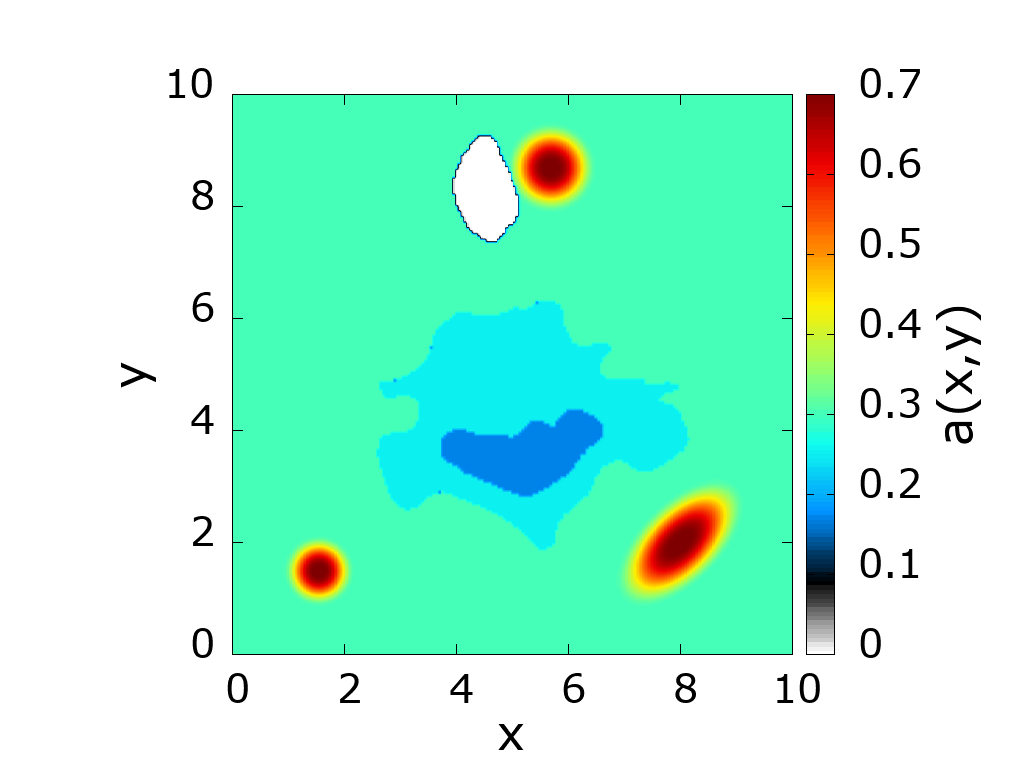
\includegraphics[width=0.45\textwidth]{figuras/necktrue.png}\\

  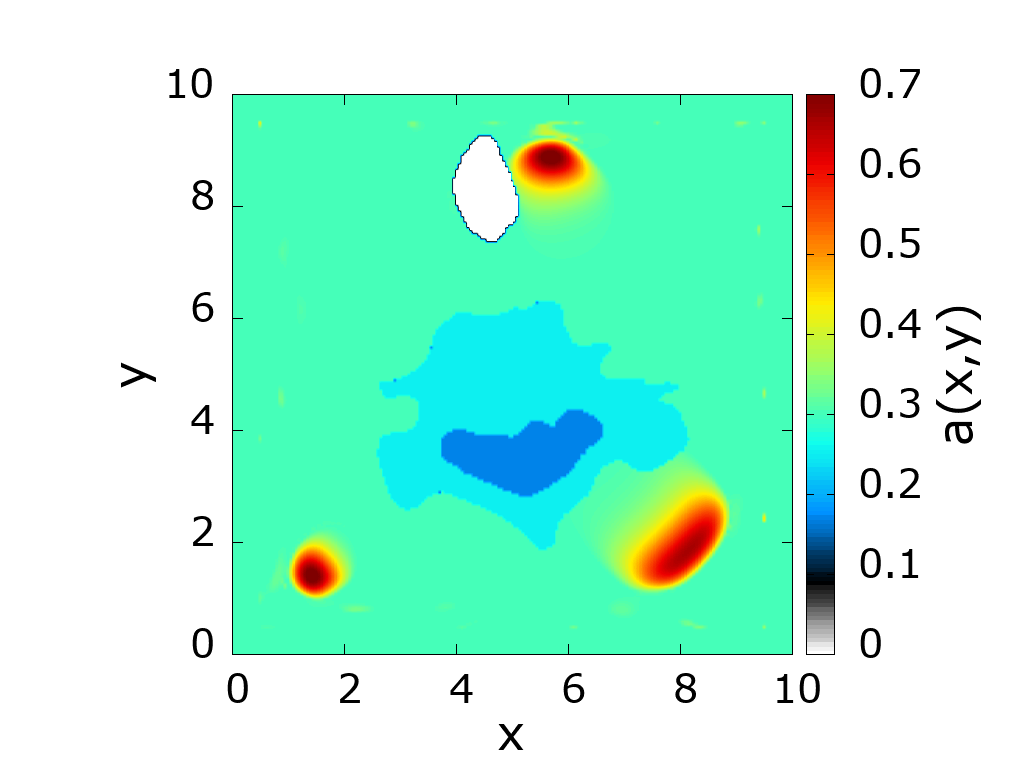
\includegraphics[width=0.45\textwidth]{figuras/necksweep.png}\\

  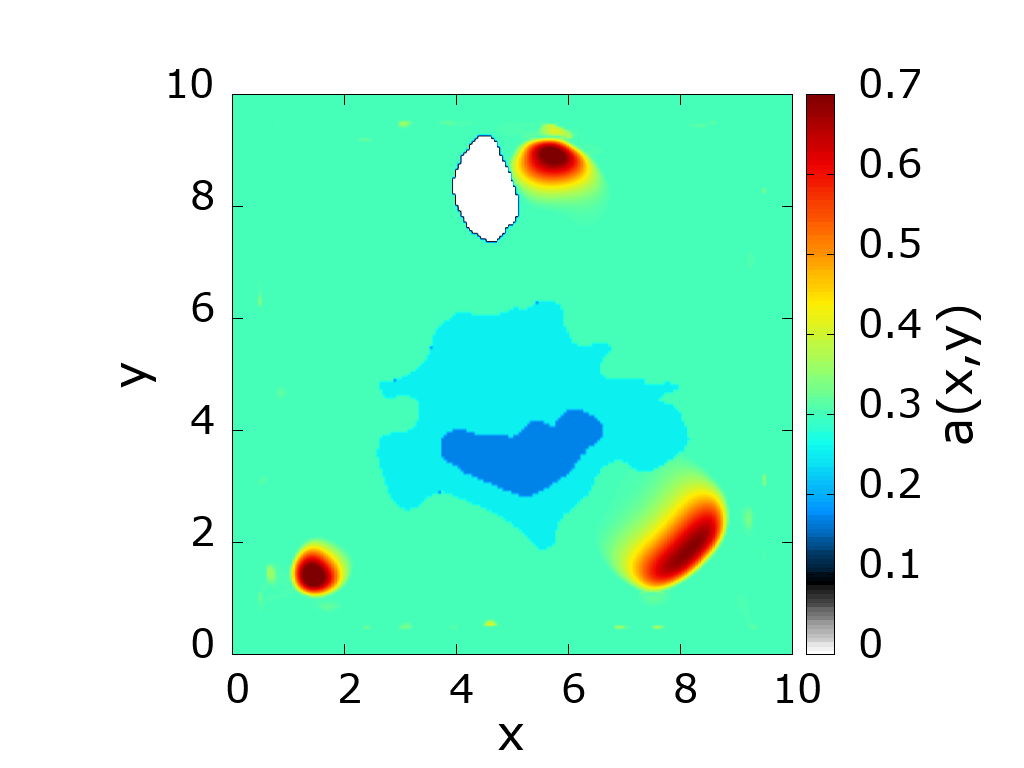
\includegraphics[width=0.45\textwidth]{figuras/neckmss.png}
  \caption{De arriba a abajo: coeficiente de absorción verdadero, y
  coeficientes de absorción obtenidos mediante resolución del problema inverso para 100 iteraciones de los métodos MB y FMS, respectivamente.}
 \label{fig:reconst}
\end{wrapfigure}
mayor en las reconstrucciones que el número de detectores. 
Esto puede entenderse de la siguiente manera: la función de las fuentes 
es producir los fotones que viajan a través del medio participante para sensarlo 
y finalmente ser recolectados en los detectores. 
Matemáticamente, las diferencias entre las señales simuladas y 
experimentales ($G-\widetilde{G}$) constituyen las ``fuentes'' en el problema 
adjunto~\eqref{eq:AdjointProblem}.
A su vez, la intensidad de estas fuentes virtuales depende de la cantidad 
de fotones originados por las fuentes láser que inyectan la radiación. 

En resumen, nuestras simulaciones demuestran la importancia de tener una cantidad 
de fuentes suficiente como para sensar el medio en las distintas regiones de interés. 
Dado que ambos métodos emplean idénticas fuentes, 
la cantidad total de fotones emitidos es la misma. Para una correcta 
resolución del problema inverso se requiere un número suficiente 
de fuentes, pero no es relevante si el problema directo 
se asumen fuentes independientes, o la superposición 
de las mismas. El método MB requiere la resolución del problema 
directo--adjunto por cada fuente, lo que resulta sumamente costoso 
desde el punto de vista computacional. Por el contrario, demostramos que 
es posible desarrollar una estrategia de encendido de dichas fuentes, 
que nos permite reducir considerablemente este costo, sin perjuicio 
de los resultados obtenidos. 

%Sin embargo, en el método MB sólo una parte de estos fotones aporta 
%información relevante. Por el contrario, el método FMS permite explotar 
%en todos los tiempos fotones que poseen información relevante para el proceso de inversión. 

%Si bien los detectores son necesarios para conocer la distribución de los fotones en el medio, 
%es mas importante la cantidad de fuentes que inyectan 
%radiación para sensar el medio, que si esas fuentes son simuladas en problemas 
%directos separados, lo cual sugiere que el método FMS es una estrategia 
%de optimización adecuada que permite ganar tiempo de cómputo aprovechando 
%el uso de fuentes simultáneas en único problema directo.
En la figura~\ref{fig:reconst} mostramos el coeficiente de absorción verdadero, 
junto con los coeficientes de absorción obtenidos mediante la resolución del problema 
inverso empleando las estrategias MB y FMS, con 16 fuentes y 36 detectores 
para 100 iteraciones del algoritmo~\ref{algfcinv}. Como puede observarse, 
las reconstrucciones obtenidas por ambos métodos son de similares características. 

\subsection{Imagenes de activación hemodinámica 
o tejido canceroso en modelo de cabeza humana}
Finalmente, presentaremos una reconstrucción simulando un ``modelo de cabeza''. 
Para esta demostración, utilizaremos el modelo de cabeza similar 
a los utilizados en las referencias~\cite{Klose2002,Prieto2017}. 
Este modelo de cabeza simula la situación típica donde 
se utiliza tomografía óptica para estudiar la actividad hemodinámica 
en el cerebro humano, y captura la característica más importante 
en este contexto, el cual es la región ubicada entre el cráneo y el cerebro, 
la cual contiene un fluido de baja absorción y baja dispersión, conocido 
como fluido cerebroespinal. Esta región cumple la función de 
amortiguar al cerebro ane movimientos bruscos. Además, el fluido cerebroespinal 
se encarga de transportar nutrientes hacia el cerebro, y de
eliminar metabolitos.

Dado que el fluido cerebroespinal presenta coeficientes de absorción y de dispersión 
despreciables, la ecuación de difusión de fotones no es físicamente preciso para modelar 
el transporte de fotones en esta región, por lo cual debe emplearse la ecuación de transporte.
En la referencia~\cite{Prieto2017} se utilizan 16 fuentes, 4 por cara, para 
un modelo de cabeza similar. 

 Aquí emplearemos 32 detectores, con 8 detectores por cara, 
e igual número de fuentes. 
Mostramos el coeficiente de absorción después de 50 iteraciones del método MB, 
e iteramos el método FMS hasta obtener un error de convergencia similar en la norma $L^2$~\eqref{eq:errl2}. En estas reconstrucciones, nuevamente buscamos inclusiones 
sobre un fondo conocido, el cual es utilizado como estimación inicial $a^0(\x)$. 
La región del fluido cerebroespinal, así como la región por fuera del mismo, 
se asumen conocidos (dado que en estas regiones no puede ocurrir la activación cerebral), 
y se mantienen fijos durante el proceso de reconstrucción. Buscamos las inclusiones 
en la región circular interior, dado que es en esta región donde se encontraría 
el cerebro en una situación menos idealizada.

Para mostrar que también pueden emplearse otras estrategias de activación, 
en esta prueba utilizaremos una configuración diferente para la 
activación de las fuentes en el método FMS. Todas las fuentes ubicadas 
en una misma cara serán activadas de manera simultánea~(Fig.~\ref{fig:headsrcs}). 

\begin{figure}[h!]
\centering
  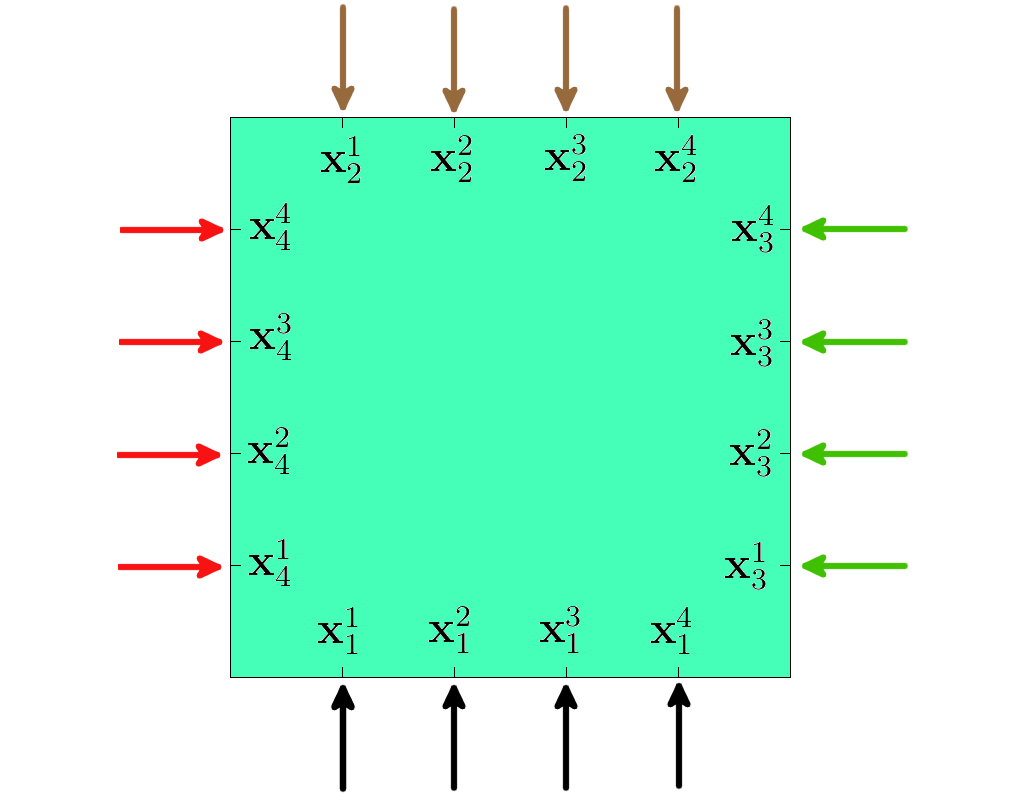
\includegraphics[width=0.5\linewidth]{figuras/head_srcs.png}\\
  \caption{Estrategia de activación de fuentes generalizadas 
  empleada para la reconstrucción en el modelo de cabeza humana. Las flechas indican la ubicación de las fuentes, 
  y los colores indican los tiempos de activación, 
  donde un mismo color indica fuentes láser que se activan 
  de manera simultanea.}
 \label{fig:headsrcs}
\end{figure}
Nuevamente, utilizamos la notación de la sección anterior, con 
$\x_k^i$, ($i=1,\ldots,4$ ~$k=1,\ldots,4$) indica la posición 
de la fuente $i$ esima activada a tiempo  $\tau_{k,1}$.
En la Tabla~\ref{tab:headsrc} se muestra la configuración de activación 
para cada conjunto de fuentes, y en la Tabla~\ref{tab:headxsrc} 
las posiciones correspondientes.

\begin{table}[h!]
\caption{Configuración de activación FMS: modelo de cabeza humana}
\vspace{-0.3cm}
\begin{center}
\begin{tabular}{cccccc}
\hline
& ~ & $\tau_{1,1}$ ~ & $\tau_{2,1}$ ~ & $\tau_{3,1}$  ~ & $\tau_{4,1}$ \\
\hline
%\hline
 & ~ & $0$ ps ~ &  $100$ ps ~ & $400$ ps ~ & $500$  \\
\hline
\end{tabular}
\label{tab:headsrc}
\end{center}
\end{table}

\begin{table}[h!]
\caption{Configuración de posiciones $\x_k^i$}
\vspace{-0.4cm}
\begin{center}
\begin{tabular}{cccccc}
\hline
%\hline
 ~ & $\x_1^1=(1.0,0.0)$ cm ~ & $\x_1^2=(2.0,0.0)$ cm ~ & $\x_1^3=(3.0,0.0)$ cm  ~ & $\x_1^4=(4.0,0.0)$ cm \\
 ~ & $\x_2^1=(1.0,5.0)$ cm ~ & $\x_2^2=(2.0,5.0)$ cm ~ & $\x_2^3=(3.0,5.0)$ cm  ~ & $\x_2^4=(4.0,5.0)$ cm \\
 ~ & $\x_3^1=(5.0,1.0)$ cm ~ & $\x_3^2=(5.0,2.0)$ cm ~ & $\x_3^3=(5.0,3.0)$ cm  ~ & $\x_3^4=(5.0,4.0)$ cm \\
 ~ & $\x_4^1=(0.0,1.0)$ cm ~ & $\x_4^2=(0.0,2.0)$ cm ~ & $\x_4^3=(0.0,3.0)$ cm  ~ & $\x_4^4=(0.0,4.0)$ cm \\
\hline
\end{tabular}
\label{tab:headxsrc}
\end{center}
\end{table}


%En la notación 
%utilizada anteriormente, tendremos $\x_1^1=(1.0,0.0)$, 
%$\x_1^2=(2.0,0.0)$, $\x_1^3=(3.0,0.0)$, $\x_1^4=(4.0,0.0)$, con retardo temporal $\tau_{1,1}=0$ps. \looseness=-1

%Luego 
%$\x_2^1=(1.0,5.0)$, 
%$\x_2^2=(2.0,5.0)$, $\x_2^3=(3.0,5.0)$,  $\x_2^4=(4.0,5.0)$ con $\tau_{2,1}=100$ps, 
%$\x_3^1=(5.0,1.0)$, 
%$\x_3^2=(5.0,2.0)$, $\x_3^3=(5.0,3.0)$,  $\x_3^4=(5.0,4.0)$ con $\tau_{3,1}=400$ps 
%y $\x_4^1=(0.0,1.0)$, 
%$\x_4^2=(0.0,2.0)$, $\x_4^3=(0.0,3.0)$,  $\x_4^4=(0.0,4.0)$ con retardo temporal de $\tau_{4,1}=500$ps.
En la figura~\ref{fig:ithead} mostramos la evolución del error ec.~\eqref{eq:errl2} 
para los métodos MB y el método FMS propuesto. En la figura~\ref{fig:rechead} 
mostramos el coeficiente de absorción verdadero, y los obtenidos al final 
de la iteración para cada método.
\begin{figure}[h!]
\centering
  \includegraphics[width=0.5\linewidth]{figuras/l2err.eps}\\
  \caption{Evolución del error en la norma $L^2$ por iteración ec.~\eqref{eq:errl2} para el coeficiente de absorción, obtenido para el modelo de cabeza humana para los métodos MB y FMS.}
 \label{fig:ithead}
\end{figure}


En términos de tiempo computacional, las cincuenta iteraciones del método 
MB tomaron mas de seis veces que las setenta y nueve iteraciones del 
método FMS. Si los dos métodos fueran iterados igual número de iteraciones, 
se obtendrían reconstrucciones similares, con un detrimento en favor 
del método MB, pero con el método FMS realizando las iteraciones en casi un órden 
de magnitud más rápido. La calidad de las reconstrucciones han mostrado 
depender en la discretización numérica utilizada. En particular, 
si se utilizan menos direcciones discretas, se obtienen 
reconstrucciones de menor calidad para ambos métodos, 
posiblemente debido a la aparición del efecto de rayos 
en el interior de la región de baja absorción y dispersión. 
%\begin{wrapfigure}{r}{0.48\textwidth}
\begin{figure}
\centering
  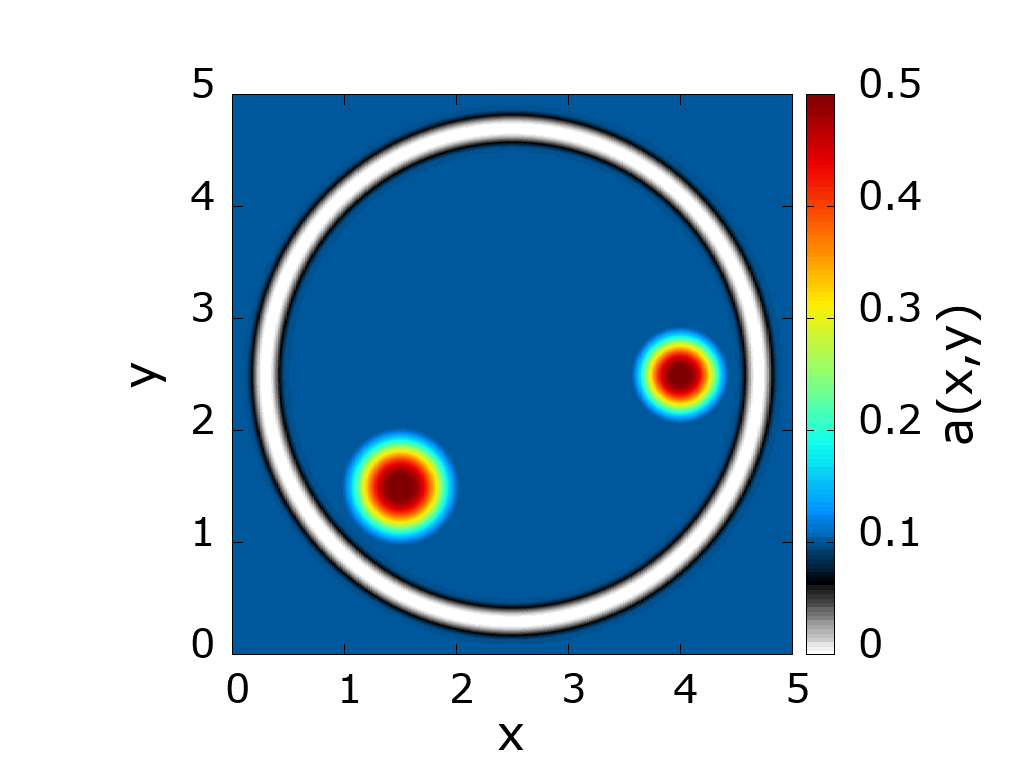
\includegraphics[width=0.32\textwidth]{figuras/head_true.png}
  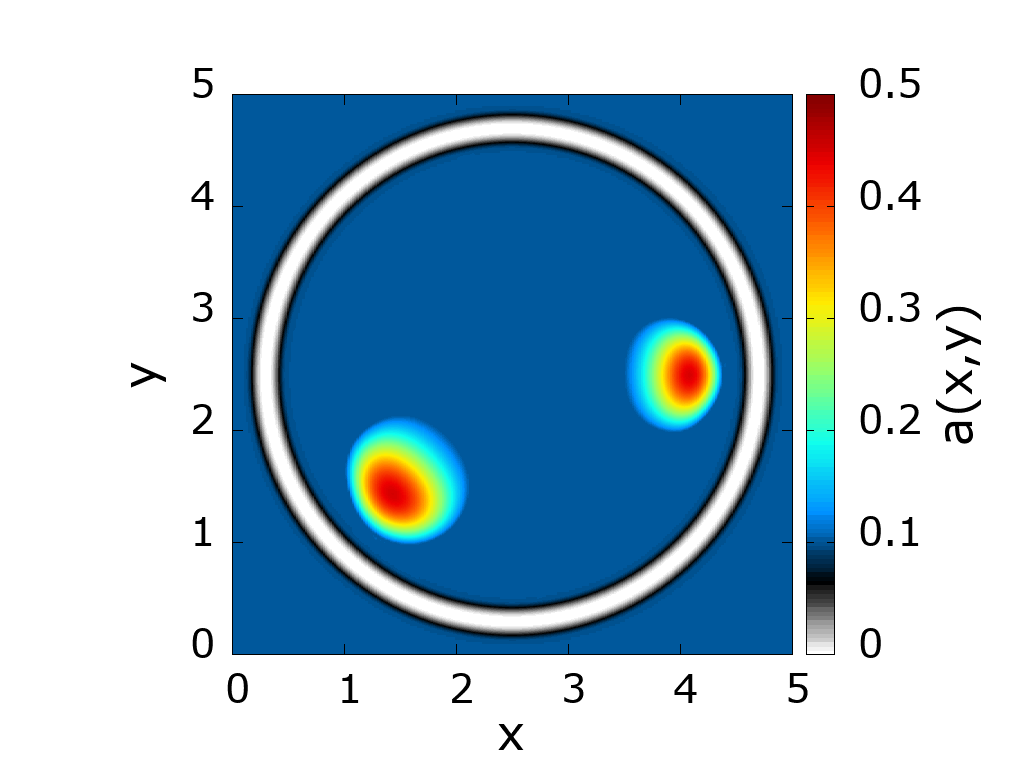
\includegraphics[width=0.32\textwidth]{figuras/head_sweep.png}
  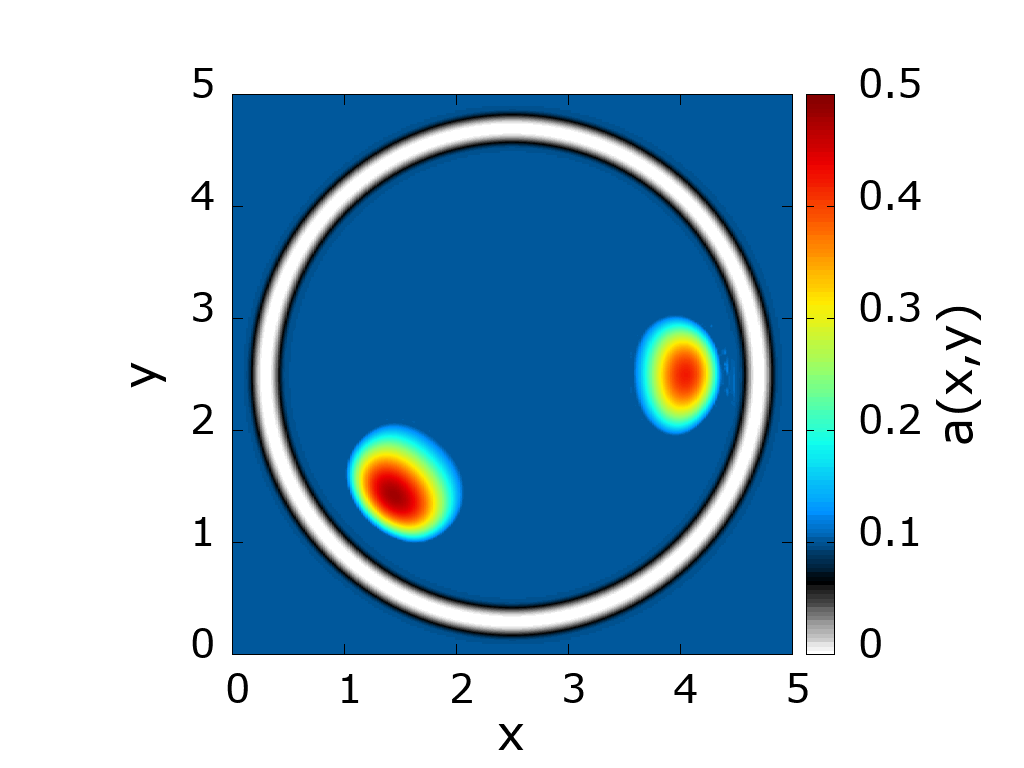
\includegraphics[width=0.32\textwidth]{figuras/head_ours.png}
%  \caption{De arriba a abajo: coeficiente de absorción verdadero, y coeficientes de 
  \caption{Izquierda a derecha: coeficiente de absorción verdadero, y coeficientes de 
  absorción obtenidos para 50 iteraciones del método MB, y 79 iteraciones del métofo FMS.}
 \label{fig:rechead}
\end{figure}
%\end{wrapfigure}
También es posible emplear otras estrategias de activación en el método 
FMS. A pesar de que no hemos explorado otras posibilidades, 
es posible incluir más fuentes generalizadas, con diferentes 
estrategias de activación para cada una de ellas. 

\pagestyle{empty}

